% \RequirePackage{fix-cm}
% \documentclass[smallcondensed]{svjour3}
% \smartqed
% \usepackage{natbib}
% \usepackage{amsmath,amssymb,amsfonts}
% \usepackage{graphicx}
% \usepackage{textcomp}
% \usepackage{xcolor}
% \usepackage{algorithm}
% \usepackage{algpseudocode}
% \usepackage{booktabs}
% \usepackage{multirow}
% \usepackage{adjustbox}
% \usepackage{float}
% \usepackage{bm}

% \newtheorem{proposition}{Proposition}
% \newtheorem{remark}{Remark}

% \journalname{Applied Intelligence}

% \def\BibTeX{{\rm B\kern-.05em{\sc i\kern-.025em b}\kern-.08em
%     T\kern-.1667em\lower.7ex\hbox{E}\kern-.125emX}}

% \begin{document}

% \title{SCoPE: A Soft-Coupled Parallel-Decoding Framework for Dynamic Weapon-Target Assignment}
% \titlerunning{SCoPE: Soft-Coupled Parallel Decoding for DWTA}

% \author{Jaejin Lee}

% \institute{Jaejin Lee \at
%   Intel Corporation, Chandler, AZ 85226, USA \\
%   \email{jaejin.lee@intel.com}
% }

% \date{Received: date / Accepted: date}

% \maketitle

% \begin{abstract}
% The Dynamic Weapon-Target Assignment Problem (DWTAP) is a critical and computationally challenging optimization problem in defense operations. We propose SCoPE (Soft-COupled Parallel-decoding framework for wEapon-target assignment), a reinforcement learning framework that integrates a modified transformer architecture with beam search and rollout-based planning. %% TODO: abstract content itself (results numbers, framing) still describes the old sequential-decoder work -- rewrite last, once A/B/C/D results are finalized. Unlike purely greedy policies, SCoPE enhances inference by combining beam search exploration with two rollout strategies: pure rollout for smaller instances and truncated neural rollout for larger problems, thereby balancing solution quality and computational efficiency.

% SCoPE is trained using parallel multi-episodic REINFORCE on small-scale instances (5 weapons, 5 targets, 5 time steps) and generalizes effectively to significantly larger instances of up to 10×10×10 configurations. The framework incorporates realistic battlefield constraints including weapon reload times, ammunition limitations, and target availability windows across multiple time stages. Experimental results demonstrate that SCoPE achieves scalable real-time inference through greedy execution, while beam search with rollout improves solution quality with manageable computational overhead. Compared to commercial solvers, SCoPE maintains performance gaps of 6--17\% while achieving substantially faster inference times. These findings highlight SCoPE as an effective and scalable framework for dynamic assignment problems requiring both accuracy and real-time decision-making capability.

% \keywords{Reinforcement learning \and Multi-agent coordination \and Combinatorial optimization \and Dynamic weapon-target assignment \and Transformer}
% \end{abstract}

% \section{Introduction}
% \label{sec:introduction}

% \PARstart{T}{he} term Operational Research (OR) was first coined in 1940 by A.P. Rowe, a scientist at the British Air Ministry~\cite{kirby2003operational}. During World War II, the British formed teams of scientists, mathematicians, and engineers tasked with analyzing and optimizing military operations. These teams addressed critical challenges such as optimizing bomber tactics~\cite{kirby2003operational}. Within this context, the Weapon-Target Assignment Problem (WTAP) emerged as a central modeling challenge for defense applications. First proposed by Manne in 1958~\cite{manne1958target}, the WTAP has since remained an active research topic due to its relevance in diverse battlefield and strategic scenarios~\cite{ahuja2007exact}.

% The WTAP seeks to assign a set of weapons to a set of targets to minimize the expected residual value of the targets after engagement. In its original static form, the WTAP involves a one-time allocation of weapons of type $m \in M$ to targets $n \in N$, where each target has an associated value $V_n$, each weapon type has a limited inventory $A_m$, and the effectiveness of weapon-target pairings is characterized by a damage rate $P_{m,n}$.

% This paper extends the static WTAP into a Dynamic Weapon-Target Assignment Problem (DWTAP) by incorporating multiple time frames ($T > 1$) and operational constraints such as target availability windows and weapon reload times. In realistic combat settings, targets may only be exposed during specific intervals, and weapon systems often require reloading or maintenance between engagements. Modeling these temporal dynamics provides a richer and more practical representation of battlefield scenarios, allowing for adaptive decision-making over time. The full mathematical formulation of DWTAP is presented in Section~\ref{sec:problem}.

% %% TODO: motivate the real-time, repeated-decision nature of DWTAP (engagement windows
% %% close quickly; re-planning must keep pace, cf. the OODA decision-cycle framing already
% %% used in the receding-horizon DWTA literature~\cite{zhang2020efficient,zhang2020dynamic}).
% %% Find/justify a WTA-appropriate time budget from the defense literature -- do NOT reuse
% %% the 120s figure from the semiconductor companion paper~\cite{lee2026litho} without an
% %% independent, domain-specific justification. Deferred; revisit before submission.

% Due to its combinatorial structure, the WTAP belongs to the class of NP-hard problems~\cite{lloyd1986weapons}, implying that computational complexity grows rapidly with problem size. As with other classical NP-hard problems such as the Traveling Salesman Problem and the Vehicle Routing Problem, two main categories of approaches have been employed: exact optimization~\cite{ahuja2007exact,johansson2011mixed,lee2019real} and approximate methods~\cite{lee2003genetic,karasakal2009efficient,li2021novel}. Exact approaches guarantee optimality but are computationally infeasible for large-scale instances, while heuristics and metaheuristics offer faster solutions but often rely on domain-specific customization, limiting their adaptability.

% In response, reinforcement learning (RL) has emerged as a promising alternative. Unlike handcrafted heuristics, RL methods learn adaptive policies that generalize across different instances and scales. Recent advances in neural combinatorial optimization have demonstrated that RL can compete with or outperform classical heuristics and metaheuristics on a variety of assignment and scheduling problems~\cite{lee2024attention,kool2018attention,kwon2020pomo}.

% In this work, we introduce SCoPE (Soft-COupled Parallel-decoding framework for wEapon-target assignment), a transformer-based RL framework for solving the DWTAP. Our method employs a modified transformer architecture to embed MDP states and trains the policy using parallel multi-episodic REINFORCE. To further enhance solution quality at inference, we integrate rollout-enhanced planning with beam search, including a truncated neural rollout that balances solution quality with computational efficiency.

% The main contributions of this study are summarized as follows:

% \begin{itemize}
%     \item \textbf{Realistic dynamic battlefield modeling}: Extension of WTAP to dynamic settings with multiple time steps, weapon reload constraints, ammunition limits, target availability windows, and weapon-target engagement compatibility ($Q_m$), reflecting platform-level operational restrictions absent from prior DWTAP formulations.

%     \item \textbf{A structural distinction for multi-agent combinatorial optimization}: We characterize DWTAP as a \emph{soft-coupled} multi-agent assignment problem, in which coordination among weapons arises from the nonlinear, multiplicative structure of the objective (Eq.~\eqref{eq:objective_function}) rather than from hard resource exclusivity as in routing- and scheduling-style multi-agent problems~\cite{parco2024}. We show that a parallel multi-pointer decoder without an explicit, learned conflict-resolution mechanism is sufficient to induce coordinated, non-wasteful target engagement in this setting.

%     \item \textbf{Rigorous, standardized benchmarking}: SCoPE is trained on a small-scale multi-scale curriculum but generalizes effectively to significantly larger held-out instances, evaluated across four size tiers up to $70 \times 100 \times 15$. We evaluate against exact (SCIP), classical heuristic, metaheuristic, and standard neural combinatorial optimization baselines under a multi-seed, statistically reported evaluation protocol.

%     \item \textbf{Rollout-enhanced inference}: Building on rollout algorithms~\cite{bertsekas1997rollout} and simulation-guided beam search~\cite{choo2022sgbs}, we adapt beam search with pure and truncated neural rollout to DWTAP's time-windowed, resource-constrained action space, improving solution quality over greedy selection while offering a tunable trade-off between performance and runtime.
% \end{itemize}

% The remainder of this paper is organized as follows: Section~\ref{sec:related} reviews related work, Section~\ref{sec:problem} presents the problem formulation, Section~\ref{sec:mdp} details the MDP formulation, Section~\ref{sec:method} describes the proposed SCoPE methodology, Section~\ref{sec:results} reports experimental results, and Section~\ref{sec:conclusion} concludes with insights and future directions.

% \section{Related Work}
% \label{sec:related}

% The Weapon Target Assignment Problem (WTAP) was first introduced by~\cite{manne1958target} as a nonlinear integer programming problem in the operations research community and has since been actively researched due to its significant applicability in the military domain. Lloyd and Witsenhausen~\cite{lloyd1986weapons} demonstrated that the WTAP is an NP-hard problem. Until the 1970s, primary research focused on transforming the original WTAP into a solvable approximation problem, i.e., converting a nonlinear programming problem into a linear programming problem~\cite{day1966allocating,firstman1960approximating,hodson1971linear,bracken1968selected,manne1958target,denbroeder1959optimum} by relaxing the nonlinear objective function and simplifying certain conditions, such as assuming that all weapons are identical~\cite{manne1958target,denbroeder1959optimum}. However, this oversimplified scenario fails to effectively capture the complexities of real battlefield environments.

% Recent studies have sought to address WTAPs without such simplifications to better reflect real battlefield situations, mainly in two directions: (1) exact solution approaches and (2) heuristic approaches. For the exact solution approach, empirical experiments were conducted in~\cite{johansson2009empirical} to determine the limit of the configuration of weapons and targets using exhaustive search. This study showed that the original WTAP can be solved within 15 minutes with nine weapons and eight targets, but it cannot be solved within an hour if one additional weapon or target is added. Kline et al.~\cite{kline2019weapon} utilized a branch-and-bound algorithm to solve a problem with 10 weapons and 10 targets of the original static WTAP. However, when the problem size increased, the computation failed to converge within seven days, demonstrating the challenge posed by this NP-hard problem. A notable study on the exact solution approach was conducted by Ahuja et al.~\cite{ahuja2007exact}, who proposed an exact algorithm to solve the original static WTAP using three different lower bounds with branch-and-bound algorithms. This study achieved global optimal solutions for up to 80 weapons and 80 targets in the original static WTAP within 24 hours. This seminal research turned medium-sized problems, previously considered unsolvable, into problems solvable optimally. Despite extensive research into exact solution approaches, no algorithms have yet been identified that can optimally solve large-scale variants of the original WTAP and DWTAP. This challenge has led researchers to focus on heuristic algorithms instead.

% Various heuristics and metaheuristics have been developed to address the WTAP. Methods such as the maximum marginal return, proposed by Kolitz and Eckler~\cite{kolitz1988analysis}, along with genetic algorithms, ant colony optimization, and simulated annealing~\cite{lee2002immunity,lee2003efficiently,durgut2017artificial,sonuc2017parallel,chang2018solving,metler1990suite}, aim to find good solutions in real-time. However, these methods often depend heavily on specific problem structures, which limits their effectiveness when applied to problems with different constraints and often necessitates development from scratch.

% To address these issues, researchers have begun applying learning-based algorithms to WTAP, inspired by the success of machine learning in various domains. For static WTAPs (SWTAPs), Wacholder~\cite{wacholder1989neural} introduced the first machine learning-based algorithm for the original WTAP using a neural network, marking a new avenue to apply learning-based approaches to WTAP. However, the method presented in this study has limitations due to its model structure, making the trained model applicable only to instances of the same size as those used during training.

% Meng et al.~\cite{meng2021deep}, Shin et al.~\cite{shin2020mean}, and Luo et al.~\cite{luo2021learning} applied deep Q-learning to static WTAP variants, broadening its scope to hypersonic missile targeting, radar-to-target assignment, and cost-aware formulations. However, the approaches of Shin et al.~\cite{shin2020mean} and Meng et al.~\cite{meng2021deep} suffer from the limitation that their neural network structures are still contingent on problem size, restricting their scalability and generalization. While Luo et al.~\cite{luo2021learning} proposed a model that utilizes a fixed number of input and output nodes, allowing it to handle problem sizes different from those encountered during training, the approach lacks several critical real-world constraints, such as ammunition limitations and target time windows.

% Na and Choi~\cite{na2023weapon} employed an actor-critic algorithm with a pointer network~\cite{vinyals2015pointer}, incorporating an attention mechanism similar to our state representation approach. Their method achieved impressive results compared to the mixed integer linear programming approach. However, a major drawback is the oversimplification that all weapons are assumed to be identical.

% Gaudet, Drozd, and Furfaro~\cite{gaudet2023} developed a deep reinforcement learning framework for optimizing weapons-to-target assignment in hypersonic strikes, utilizing Proximal Policy Optimization. Their approach demonstrated near-optimal performance with a 1000$\times$ speedup compared to traditional nonlinear integer programming methods. However, their policy network is designed to handle a maximum of only 12 weapons and 20 targets, limiting its scalability to larger, more complex scenarios.

% Regarding DWTAPs, most existing work simplifies the problem to maintain tractability. Zhang et al.~\cite{zhang2020efficient,zhang2020dynamic} decomposed a DWTAP into sequential SWTAPs solved at each time stage via a receding-horizon heuristic, assuming that solving each stage independently and near-optimally approximates the global optimum. Although this simplification makes each engagement more manageable by treating stages independently, it overlooks the interconnected nature of warfare solutions and does not leverage a learned, generalizable policy. In contrast, our approach solves DWTAP as a single multi-stage decision process without decomposing across time, using reinforcement learning to capture cross-stage dependencies while incorporating realistic military operation scenarios.

% Wu et al.~\cite{wu2022dynamic} introduced a dynamic target assignment model that assumes a specific use case involving ballistic missiles targeting a group of targets. They effectively linked the model to wargame simulations, providing a meaningful use case. They utilized a soft actor-critic reinforcement learning model. However, one limitation of their model is that its network structure depends on the number of weapons and targets. This dependency makes the model not size-agnostic, requiring retraining for each specific configuration.

% Yoon, Lee, and Cho~\cite{yoontransformer} presented a transformer-based RL framework for scalable dynamic WTA (DWTA). %% TODO: this paragraph's description (DQN/Actor-Critic, "not scalable") describes the OLD Master's-thesis version of this work; verify it still matches the peer-reviewed journal version now cited and rewrite the comparison accordingly before submission.

% Hu, Zhang, Luo, and Chen~\cite{hu2024} applied multi-agent reinforcement learning (RL) for dynamic target assignment in Unmanned Surface Vehicles (USVs). They proposed a multi-agent actor-critic method that encodes state information using a recurrent neural network and an attention mechanism while employing multi-layer perceptrons for the policy and value networks. This approach is similar to ours in that it encodes the state in a higher dimension. However, their problem is significantly simpler than ours, as they assume all USVs are identical and their objective function does not have the nonlinearity typical of WTAP.

% DWTAP reflects more realistic battlefield scenarios than SWTAP by allocating available assets across the phases of an operation toward a desired end state, through the integration of time dynamics. Despite the critical importance of DWTAP in capturing these dynamics, the limited research in this field motivates us to explore an effective solution framework that can address DWTAP at scale and in real time.

% \subsection{Inference-Time Search for Neural Combinatorial Optimization}

% Beyond training a construction policy, recent work improves solution quality at inference time without retraining. Rollout algorithms, introduced by Bertsekas et al.~\cite{bertsekas1997rollout}, use a base policy to estimate the cost-to-go of candidate actions through simulation, guaranteeing improvement over the base policy under mild conditions. Choo et al.~\cite{choo2022sgbs} combined this idea with beam search in simulation-guided beam search (SGBS), guiding a fixed-width tree search using both policy confidence and rollout simulation on routing problems, while Hottung et al.~\cite{hottung2022eas} instead adapt policy parameters per instance at test time. The beam-search-with-rollout inference strategy used in this work (Section~\ref{sec:method}, Section~\ref{sec:method}-D) builds directly on this line of work, adapting it to DWTAP's time-windowed, resource-constrained action space; it is a tool we employ rather than a claimed algorithmic contribution of this paper.

% \subsection{Multi-Agent Combinatorial Optimization}

% A separate line of work addresses problems in which multiple agents must act jointly at each decision epoch. Learned inter-agent communication has a long history in multi-agent RL: Sukhbaatar and Fergus~\cite{sukhbaatar2016commnet} introduced CommNet, in which agents broadcast and average learned messages, and Das et al.~\cite{das2019tarmac} introduced TarMAC, which uses attention so that each agent learns whom to address. Combined with pointer-network-style output heads~\cite{vinyals2015pointer}, these communication mechanisms provide a standard, general-purpose basis for simultaneous multi-agent action selection. Park et al.~\cite{park2021schedulenet} and Hu et al.~\cite{hu2024} apply multi-agent RL to scheduling and asset-assignment problems, respectively, but assume simple, identical-agent settings.

% Building on this lineage, Berto et al.~\cite{parco2024} recently proposed PARCO for multi-agent combinatorial optimization, combining transformer-based inter-agent communication and simultaneous multiple-pointer decoding with an additional, learned priority-based \emph{conflict handler} that resolves contention when multiple agents compete for the same resource (e.g., a shared customer node in vehicle routing). This conflict-resolution mechanism is PARCO's central addition beyond prior communication-based multi-agent architectures, and it is designed specifically for \emph{hard-coupled} problems, in which simultaneous access to a resource is infeasible by construction.

% DWTAP is structurally different: multiple weapons may legally engage the same target simultaneously, so there is no hard exclusivity to resolve. Instead, coordination in DWTAP arises from the nonlinear, multiplicative structure of the objective (Eq.~\eqref{eq:objective_function}), where the marginal value of an additional hit on an already-targeted asset diminishes — a \emph{soft-coupled} coordination problem driven by the shared objective rather than by discrete feasibility. This distinction motivates the architecture in Section~\ref{sec:method}: rather than adopting PARCO's conflict handler, we build on the standard communication-and-simultaneous-pointer-decoding lineage~\cite{sukhbaatar2016commnet,das2019tarmac,vinyals2015pointer} directly, and empirically test whether this simpler mechanism, without any explicit conflict resolution, is sufficient to induce efficient, non-wasteful target coverage in a soft-coupled setting (Section~\ref{sec:results}). PARCO thus serves as our point of comparison for the hard-coupled case rather than as a component we extend.

% Note that the softness of this coupling has a second, distinct consequence beyond motivating a simpler architecture: it also bounds the \emph{cost} of imperfect coordination. Because all $M$ weapons in our decoder commit simultaneously from a single shared pre-round state (Section~\ref{sec:parallel-decoder}), none can observe another's choice within the same round before acting -- unlike a sequential, one-weapon-at-a-time policy, which can condition each pick on the others already made that round. This is a genuine informational disadvantage, and it is visible empirically (Section~\ref{sec:results}): per-round target dispersion is comparable between the two decoders at Small scale (84.8\% parallel vs.\ 84.2\% sequential) but the parallel decoder falls increasingly behind as scale grows, reaching a 7.8-percentage-point deficit at both Large (50.2\% vs.\ 58.0\%) and Battlefield (42.1\% vs.\ 50.0\%) scale. However, not all of this redundancy reflects wasted effort -- concentrating fire on a target that still has substantial remaining value is a legitimate strategic choice, not a coordination failure. Separating redundant hits by whether the target's pre-round survival probability was already below 20\% (i.e.\ genuinely \emph{wasteful} redundancy, as opposed to justified concentration on a still-valuable target) narrows this gap considerably: 8.2\% vs.\ 4.9\% wasteful-redundancy rate at Large scale and 7.5\% vs.\ 6.9\% at Battlefield scale, a much smaller difference than the raw dispersion numbers suggest. Consequently, the resulting gap in final destruction ratio between the two decoders stays under 2 percentage points at every tier (largest gap: 1.7 points, Large scale) despite dispersion gaps of up to 7.8 points. We view this as further evidence that DWTAP's soft coupling is precisely what makes a communication-only, conflict-handler-free architecture viable: even where simultaneous decoding coordinates imperfectly, the objective's own tolerance for redundancy limits the resulting loss. Section~\ref{sec:submodular} formalizes this intuition, deriving a worst-case bound on that loss from the submodularity of the DWTAP objective itself.

% \subsection{Neural Construction Architectures for Assignment-Structured and Large-Scale Problems}

% Beyond routing-specific architectures built around Euclidean coordinates, recent neural construction methods target problems defined by an arbitrary cost or compatibility matrix. Kwon et al.~\cite{kwon2021matrix} proposed MatNet, which directly encodes an asymmetric cost/compatibility matrix through dual-graph attention between two node types, achieving strong results on flexible flow-shop scheduling and asymmetric TSP without relying on coordinate-based embeddings. DWTAP's damage-rate matrix $P_{m,n}$ and engagement-compatibility sets $Q_m$ are naturally suited to this matrix-encoding view, and we adopt a related encoding for weapon-target compatibility (Section~\ref{sec:method}). Separately, Luo et al.~\cite{luo2023lehd} introduced a heavy-decoder architecture (LEHD) explicitly designed to generalize from small training instances to substantially larger test instances, directly relevant to SCoPE's own train-small/test-large protocol (Section~\ref{sec:results}-A); we compare against this scale-generalization behavior in our evaluation. Grinsztajn et al.~\cite{grinsztajn2023winner} further show that training a population of diverse policies, rather than a single policy, improves robustness across problem distributions, which informs our multi-seed evaluation protocol (Section~\ref{sec:results}). To standardize evaluation across these methods, we build our benchmarking pipeline (Section~\ref{sec:results}) on the RL4CO library~\cite{berto2023rl4co}, which provides reference implementations of AM~\cite{kool2018attention}, POMO~\cite{kwon2020pomo}, and related baselines under a unified training and evaluation protocol; recent surveys~\cite{mazyavkina2021reinforcement,bogyrbayeva2024survey} further contextualize the rapid growth of this subfield.

% \section{Problem Formulation}
% \label{sec:problem}

% Unlike static WTAP, the proposed Dynamic Weapon-Target Assignment Problem (DWTAP) is structured across discretized time steps, denoted as $t = 1, 2, \ldots, T$. In each time step $t$, at most one round of ammunition from each weapon $m$ can be assigned to a target $n$. This discretization enables the model to incorporate the dynamics of the battlefield and the availability of resources at each specific interval, thereby facilitating the sequential decision-making process. Within this framework, we consider realistic combat scenario constraints, such as weapon reload time, ammunition limitation, and target time windows.

% The objective is to minimize the total remaining target values, each denoted as $V_n$, by optimally assigning a set of weapons, denoted as $M$ (where $m = 1, 2, \ldots, M$), to a set of targets represented by $N$ (where $n = 1, 2, \ldots, N$). The assignment must adhere to the following constraints:
% \begin{itemize}
%     \item Each weapon $m$ can assign at most one round of ammunition to one target $n$ at each time step $t$, but multiple rounds from different weapons can be assigned to a single target simultaneously.
%     \item Each weapon, denoted as $m$, has a specified reload time $D_m$. After engaging a target, weapon $m$ must wait $D_m$ time units before it can be used again.
%     \item Each weapon $m$ has a limited amount of ammunition, represented by $A_m$, which must last across all time steps. Therefore, at any time $t$, weapon $m$ can assign ammunition only if it has not depleted its ammunition $A_m$.
%     \item Each target $n$ has a specific vulnerability window, from $t_{n, \text{start}}$ to $t_{n, \text{end}}$. A target can only be engaged during this time frame.
%     \item Each weapon $m$ has an engagement compatibility set $Q_m \subseteq N$, reflecting platform-level restrictions such as range, guidance mode, and target-type suitability; weapon $m$ may only be assigned to targets $n \in Q_m$.
%     \item The proportion of target $n$'s value reduction when hit by weapon $m$, denoted by $P_{m,n}$, quantifies how effectively weapon $m$ reduces the value $V_n$ of target $n$.
% \end{itemize}

% \subsection{Notation}
% \begin{table}[H]
% \centering
% \small
% \caption{Notations for the Mathematical Model}
% \label{tab:notation}
% \begin{tabular}{lp{6.5cm}}
% \hline
% \textbf{Sets} & \\
% $M$ & Set of weapons, indexed by $m = 1, \ldots, M$ \\
% $N$ & Set of targets, indexed by $n = 1, \ldots, N$ \\
% $T$ & Set of time stages, indexed by $t = 1, \ldots, T$ \\
% \hline
% \textbf{Parameters} & \\
% $V_n$ & Initial value of target $n$ \\
% $D_m$ & Reload time for weapon $m$ \\
% $A_m$ & Total ammunition for weapon $m$ \\
% $TW_n$ & Time window for target $n$ \\
% $Q_m$ & Engagement compatibility set for weapon $m$ ($Q_m \subseteq N$) \\
% $P_{m,n}$ & Value reduction proportion \\
% \hline
% \textbf{Decision Variables} & \\
% $x_{m,n,t}$ & Binary assignment variable \\
% $w_{m,t}$ & Remaining readiness time \\
% $a_{m,t}$ & Remaining ammunition \\
% \hline
% \end{tabular}
% \end{table}

% \subsection{Optimization Model}

% The problem can be formulated as a nonlinear integer programming problem. The objective function is:

% \begin{equation}\label{eq:objective_function}
%     \min \sum_{n=1}^{N} V_{n} \prod_{t=1}^{T} \prod_{m=1}^{M} (1 - P_{m,n})^{x_{m,n,t}}
% \end{equation}

% Subject to constraints:

% \begin{equation}\label{eq:weapon_target_constraint}
%     \sum_{n=1}^{N} x_{m,n,t} \leq 1, \quad \forall m, t
% \end{equation}

% \begin{equation}\label{eq:wait_time_update}
%     w_{m,t+1} = \max\left(0,\ w_{m,t} - 1\right) + D_{m} \sum_{n=1}^{N} x_{m,n,t}, \quad \forall m, t
% \end{equation}

% \begin{equation}\label{eq:weapon_readiness}
%     x_{m,n,t} \leq 1 - \frac{w_{m,t}}{D_{m}}, \quad \forall m, n, t
% \end{equation}

% \begin{equation}\label{eq:ammunition_usage}
%     a_{m,t+1} = a_{m,t} - \sum_{n=1}^{N} x_{m,n,t}, \quad \forall m, t
% \end{equation}

% \begin{equation}\label{eq:ammunition_constraint}
%     a_{m,t} \geq x_{m,n,t}, \quad \forall m, n, t
% \end{equation}

% \begin{equation}\label{eq:target_time_window}
%     x_{m,n,t} = 0, \quad \text{if } t \notin TW_n, \quad \forall m, n
% \end{equation}

% \begin{equation}\label{eq:compatibility_constraint}
%     x_{m,n,t} = 0, \quad \text{if } n \notin Q_m, \quad \forall m, n, t
% \end{equation}

% \begin{equation}\label{eq:binary_assignment}
%     x_{m,n,t} \in \{0,1\}, \quad \forall m, n, t
% \end{equation}

% \begin{equation}\label{eq:wait_time_integer}
%     w_{m,t} \in \mathbb{Z}_{+}, \quad \forall m, t
% \end{equation}

% \begin{equation}\label{eq:wait_time_bounds}
%     0 \leq w_{m,t} \leq D_{m}, \quad \forall m, t
% \end{equation}

% \begin{equation}\label{eq:initial_availability}
%     w_{m,1} = 0, \quad \forall m
% \end{equation}

% \begin{equation}\label{eq:remaining_ammunition_integer}
%     a_{m,t} \in \mathbb{Z}_{+}, \quad \forall m, t
% \end{equation}

% \begin{equation}\label{eq:initial_ammunition}
%     a_{m,0} = A_m, \quad \forall m
% \end{equation}

% \section{Markov Decision Process Formulation}
% \label{sec:mdp}

% The DWTAP can be modeled as a sequential decision-making problem, where a weapon is assigned to a target at each time step with the goal of minimizing the total remaining target values. This sequential decision-making process can be effectively modeled as a Markov Decision Process (MDP)~\cite{bellman1957dynamic}.

% An MDP, $M$, is represented as a 5-tuple:
% \begin{equation}
% M = (S, A, P, R, \gamma)
% \end{equation}
% where $S$ represents states, $A$ denotes actions, $P$ is the transition probability, $R$ is the reward function, and $\gamma$ is the discount factor.

% The proposed DWTAP MDP is defined as follows:

% \begin{itemize}
% \item \textbf{State ($s_t$)}: The model considers $K = M \times N + 1$ assignments. The state of each weapon-target assignment at time step $t$ is:
% \begin{equation}
% \label{eq:state}
% s_t = [u_t; v_t; d_t; r_t; a_t; f_t; ws; we; p] \in \mathbb{R}^9
% \end{equation}
% where:
% \begin{itemize}
%     \item $u_t$: Weapon readiness indicator
%     \item $v_t$: Remaining target value
%     \item $d_t$: Remaining reload time
%     \item $r_t$: Remaining time to end
%     \item $a_t$: Remaining ammunition
%     \item $f_t$: Cumulative hits on target
%     \item $ws$: Earliest attack time
%     \item $we$: Latest attack time
%     \item $p$: Value reduction proportion
% \end{itemize}

% \item \textbf{Action ($a_t$)}: Binary assignment vector of size $K$:
% \begin{equation}
%     a_t = [a_{(1,1)}, \ldots, a_{(M,N)}, a_{K}]
% \end{equation}

% \item \textbf{Transition}: Deterministic with $P(s_{t+1} | s_t, a_t) = 1$.

% \item \textbf{Reward}:
% \begin{equation}
% \label{eq:reward}
%     R(s_{t+1} | s_t, a_t) = \frac{C(s_t) - C(s_{t+1})}{C(s_{0})}
% \end{equation}
% where $C(s_t)$ is the sum of target values at state $s_t$.
% \end{itemize}

% \section{Proposed Method: SCoPE}
% \label{sec:method}

% We propose SCoPE, a reinforcement learning framework for DWTAP that encodes state as a heterogeneous weapon-target graph (Section~\ref{sec:method}-A) and decodes actions with a \emph{parallel multi-pointer} policy (Section~\ref{sec:method}-B): at every time step, all currently-live weapons choose simultaneously, each from its own compatible-target set, rather than one (weapon,target) edge being selected per network call. No explicit conflict-resolution mechanism is used -- unlike hard-coupled multi-agent construction methods such as PARCO~\cite{parco2024}, DWTAP permits multiple weapons to legally engage the same target, so coordination is hypothesized to emerge from the shared graph embeddings alone (the soft-coupling hypothesis introduced in Section~\ref{sec:related}, tested empirically in Section~\ref{sec:results}). Training uses parallel multi-episodic REINFORCE with reward-to-go and a shared parallel-rollout baseline, deliberately without a learned critic (Section~\ref{sec:method}-C reports the module-wise ablation motivating this: a critic-based value network and potential-based shaping did not improve, and in fact measurably hurt, held-out generalization for this architecture). At inference time, solution quality is further improved with beam search and rollout adapted from~\cite{bertsekas1997rollout,choo2022sgbs} (Section~\ref{sec:method}-D). Fig.~\ref{fig:overall} illustrates the overall architecture.

% \begin{figure}[htbp]
%   \centering
%   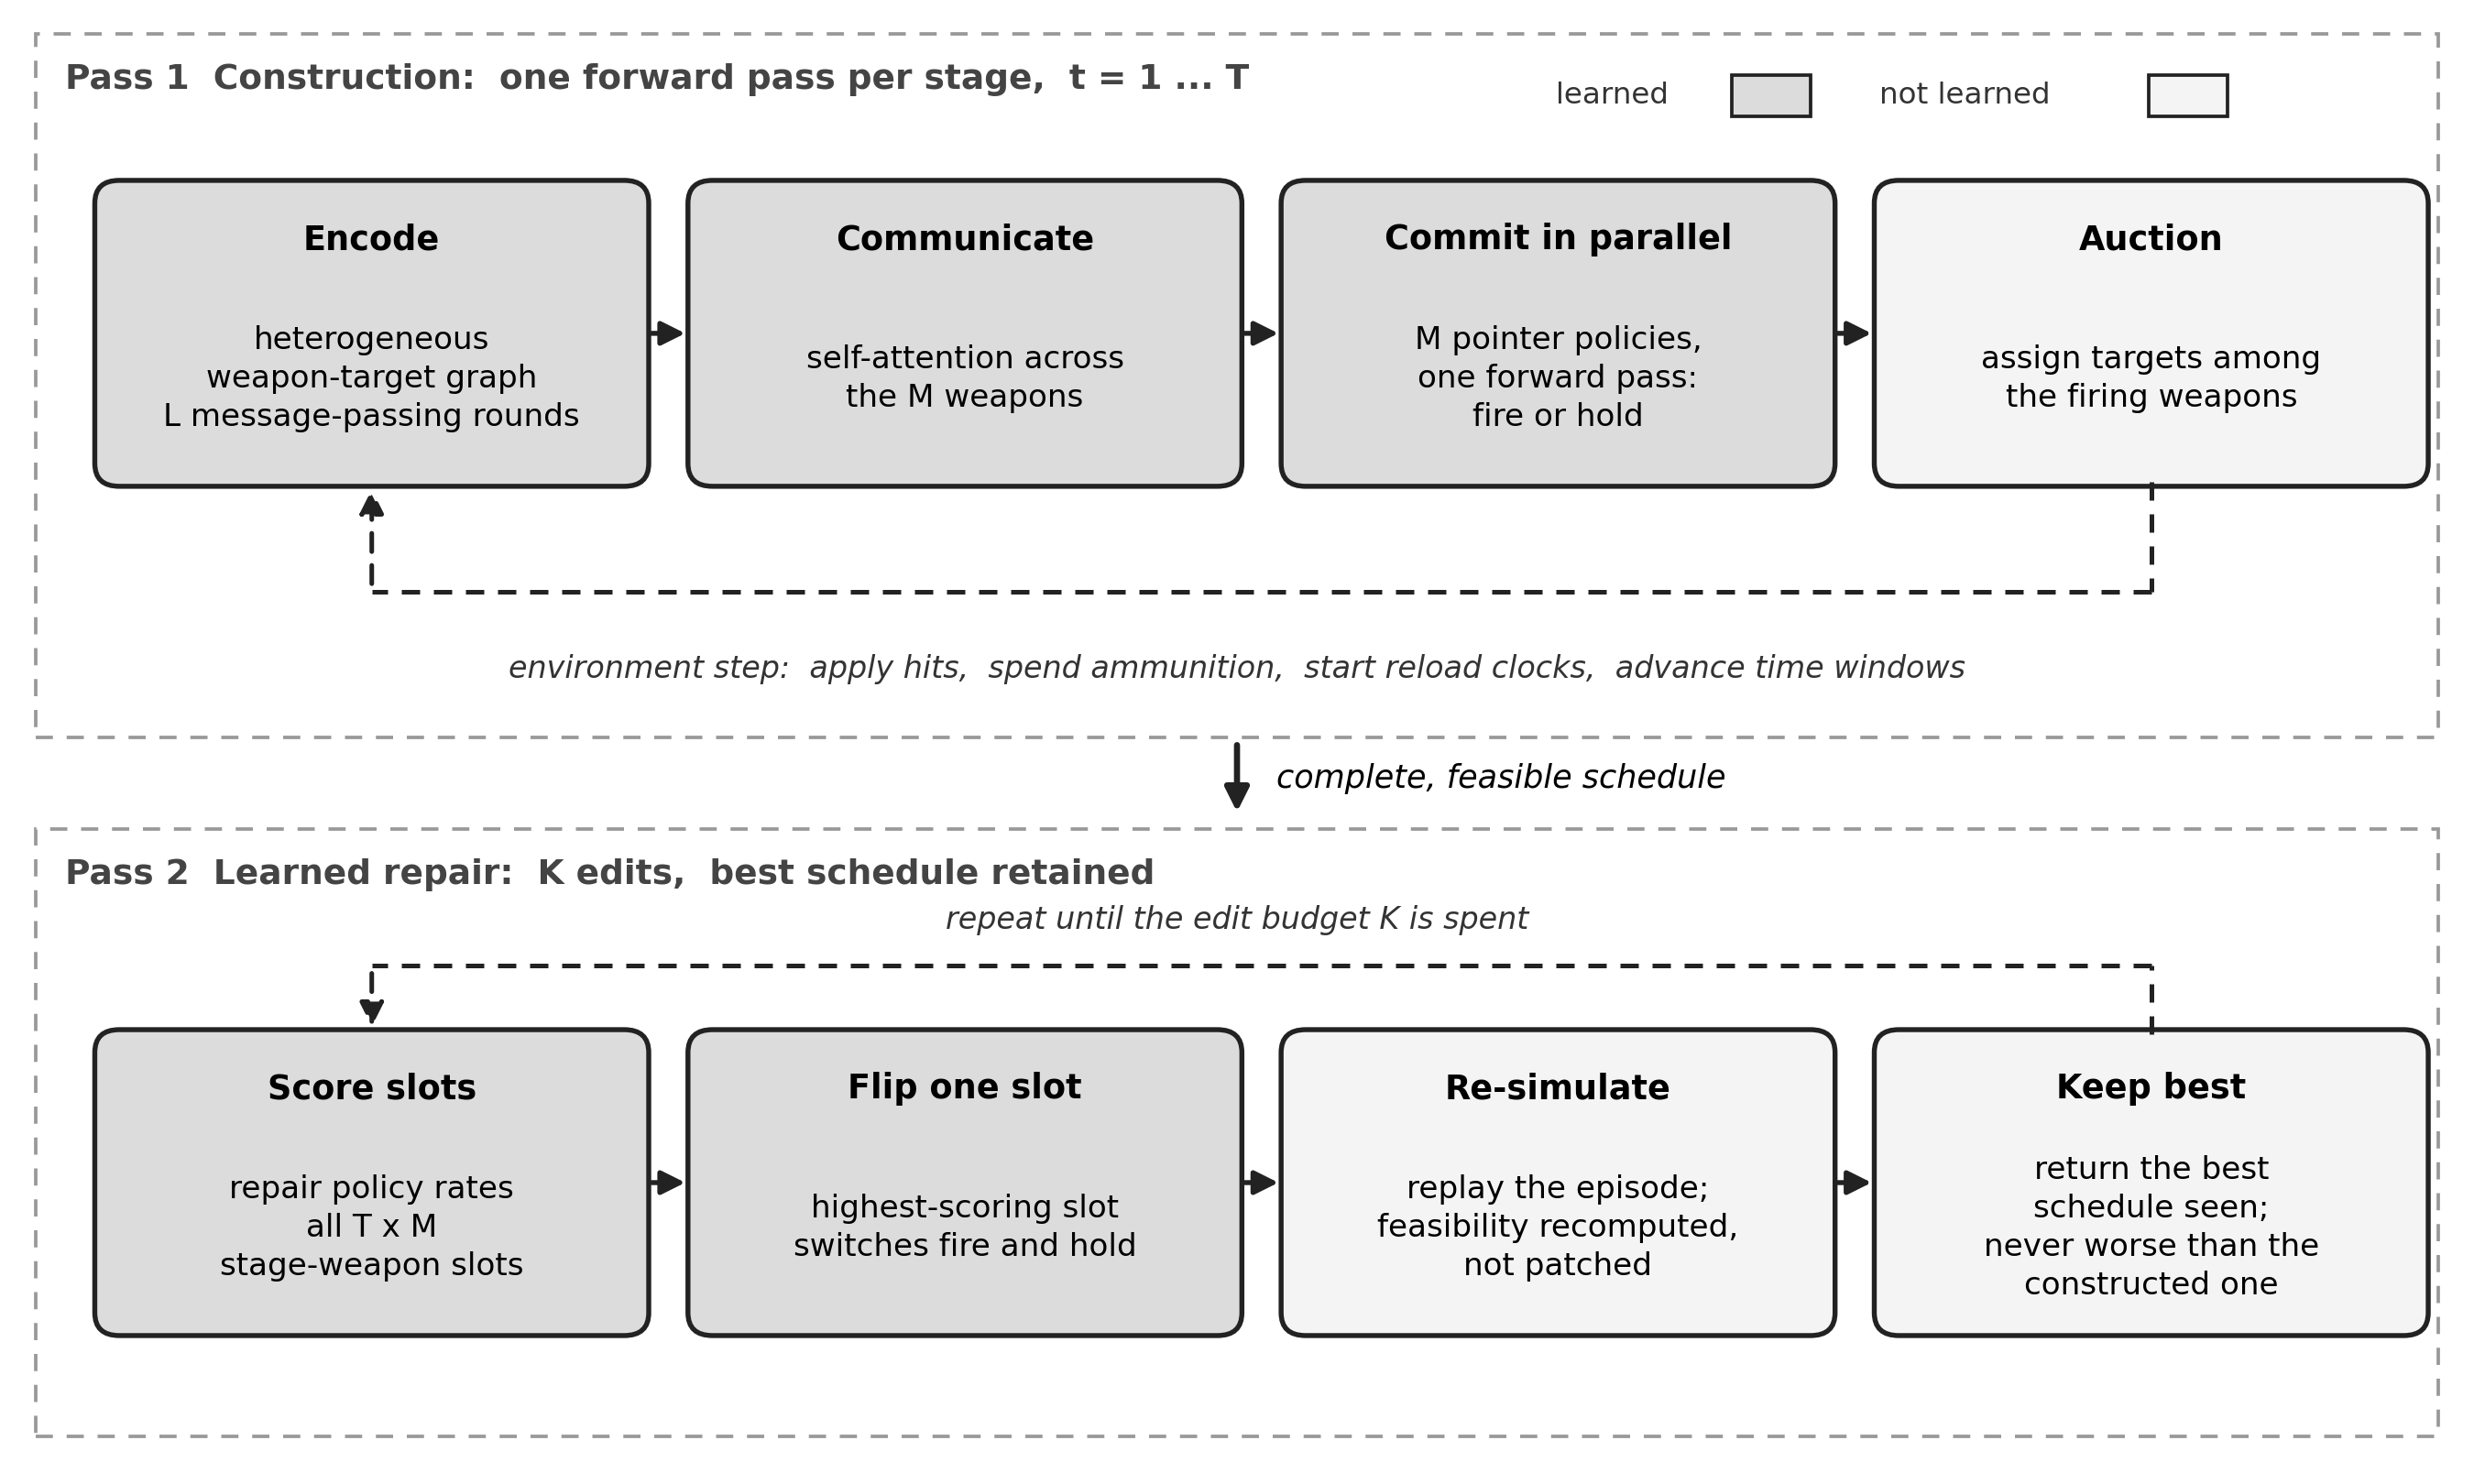
\includegraphics[width=\columnwidth]{figure/Overall.png}
%   \caption{Overall architecture of SCoPE showing training and inference processes.}
%   \label{fig:overall}
% \end{figure}

% \subsection{Heterogeneous Graph Encoding}
% \label{sec:encoding}

% The original per-pair state $\bm{s}_t = [u_t; v_t; d_t; r_t; a_t; f_t; ws; we; p] \in \mathbb{R}^9$ (Eq.~\eqref{eq:state}) decomposes naturally into three parts that do not all vary independently per (weapon,target) pair: features belonging only to weapon $m$ (readiness $u_t$, remaining reload $d_t$, remaining ammunition $a_t$), features belonging only to target $n$ (remaining value $v_t$, cumulative hits $f_t$, window bounds $ws,we$), and a single pairwise feature (damage rate $p = P_{m,n}$). We make this structure explicit with a heterogeneous graph: weapon nodes $\bm{x}_m^{\text{wpn}} \in \mathbb{R}^{4}$, target nodes $\bm{x}_n^{\text{tgt}} \in \mathbb{R}^{4}$, and edges $\bm{x}_{m,n}^{\text{edge}} \in \mathbb{R}^{1}$ carrying $P_{m,n}$, restricted to $n \in Q_m$ (Section~\ref{sec:problem}).

% Each node/edge type is linearly projected to a shared hidden dimension:
% \begin{equation}
% \bm{h}_m^{\text{wpn},(0)} = \bm{W}^{\text{wpn}}\bm{x}_m^{\text{wpn}} + \bm{b}^{\text{wpn}}, \quad
% \bm{h}_n^{\text{tgt},(0)} = \bm{W}^{\text{tgt}}\bm{x}_n^{\text{tgt}} + \bm{b}^{\text{tgt}}
% \end{equation}
% \begin{equation}
% \bm{h}_{m,n}^{\text{edge},(0)} = \bm{W}^{\text{edge}}\bm{x}_{m,n}^{\text{edge}} + \bm{b}^{\text{edge}}
% \end{equation}

% Message passing proceeds through $L$ layers. At layer $\ell$, the edge embedding is refreshed from its endpoints and its own previous value, then weapon and target embeddings aggregate messages from their incident edges via a GRU update (matching the communication mechanism of Section~\ref{sec:related}, in the lineage of~\cite{sukhbaatar2016commnet,das2019tarmac}):
% \begin{equation}
% \bm{h}_{m,n}^{\text{edge},(\ell)} = \tanh\!\left(\bm{W}_e\left[\bm{h}_m^{\text{wpn},(\ell-1)} \,\|\, \bm{h}_n^{\text{tgt},(\ell-1)} \,\|\, \bm{h}_{m,n}^{\text{edge},(\ell-1)}\right]\right)
% \end{equation}
% \begin{equation}
% \bm{h}_m^{\text{wpn},(\ell)} = \text{GRU}\!\left(\textstyle\sum_{n \in Q_m} \bm{W}_w\left[\bm{h}_m^{\text{wpn},(\ell-1)} \,\|\, \bm{h}_n^{\text{tgt},(\ell-1)} \,\|\, \bm{h}_{m,n}^{\text{edge},(\ell)}\right],\ \bm{h}_m^{\text{wpn},(\ell-1)}\right)
% \end{equation}
% and analogously for $\bm{h}_n^{\text{tgt},(\ell)}$, aggregating over weapons for which $n \in Q_m$. Because message passing runs over the full graph, every weapon's final embedding $\bm{h}_m^{\text{wpn},(L)}$ is informed by the state of every other weapon and target -- this is the channel through which coordination can occur without an explicit conflict-resolution step (Section~\ref{sec:method}-B).

% \subsection{Parallel Multi-Pointer Policy}
% \label{sec:parallel-decoder}

% Unlike a single global policy over all $M \times N$ (weapon,target) pairs (as in earlier neural WTAP/DWTAP formulations, e.g.~\cite{na2023weapon}), SCoPE decodes $M$ \emph{independent} distributions simultaneously, one per weapon, each over its own compatible targets plus a no-op:
% \begin{equation}
% \text{score}_{m,n} = \bm{w}_e^\top \, \text{Res}\!\left(\bm{h}_{m,n}^{\text{edge},(L)}\right), \quad n \in Q_m
% \end{equation}
% \begin{equation}
% \text{score}_{m,\text{noop}} = \bm{w}_0^\top \, \text{Res}\!\left(\bm{W}_0\left[\bm{h}_m^{\text{wpn},(L)} \,\|\, \bar{\bm{h}}^{\text{wpn}} \,\|\, \bar{\bm{h}}^{\text{tgt}}\right]\right)
% \end{equation}
% where $\text{Res}(\cdot)$ is a residual block, and $\bar{\bm{h}}^{\text{wpn}} = \frac{1}{M}\sum_m \bm{h}_m^{\text{wpn},(L)}$, $\bar{\bm{h}}^{\text{tgt}} = \frac{1}{N}\sum_n \bm{h}_n^{\text{tgt},(L)}$ are pooled global-context vectors, so each weapon's no-op decision is informed by system-wide state. The per-weapon policy is
% \begin{equation}
% \label{eq:parallel-policy}
% \pi_m(\cdot \mid s_t) = \text{softmax}\!\left(\left[\text{score}_{m,n}\right]_{n \in Q_m},\ \text{score}_{m,\text{noop}}\right)
% \end{equation}
% masked to targets currently available under the constraints of Section~\ref{sec:problem} (reload, ammunition, time window); no-op is always legal. All $M$ policies $\pi_1, \ldots, \pi_M$ are computed in a single forward pass and sampled independently, giving the joint action $a_t = (a_{1,t}, \ldots, a_{M,t})$ with
% \begin{equation}
% \log \pi_\theta(a_t \mid s_t) = \sum_{m=1}^{M} \log \pi_m(a_{m,t} \mid s_t).
% \end{equation}
% No learned conflict handler resolves cases where multiple weapons select the same target -- this is legal under the DWTAP constraints of Section~\ref{sec:problem}, and is precisely the soft-coupled setting distinguished from PARCO's hard-coupled design in Section~\ref{sec:related}.

% The mechanism by which coordination can nonetheless emerge is structural, not incidental. Every $\text{score}_{m,n}$ is computed from $\bm{h}_{m,n}^{\text{edge},(L)}$, which by construction (Section~\ref{sec:encoding}) has absorbed target $n$'s own embedding $\bm{h}_n^{\text{tgt},(L)}$ -- and $v_t$, target $n$'s remaining value, is one of that node's own input features $\bm{x}_n^{\text{tgt}}$. Consequently, every weapon's score for a given target is directly conditioned on that target's current state, independent of which other weapon computes it. This means the $M$ simultaneous policies $\pi_1, \ldots, \pi_M$, despite never observing one another's action this round (Section~\ref{sec:related}), are not evaluating targets from independent, uninformed priors: a target driven near zero remaining value by earlier rounds is scored low by every weapon's policy for the same reason, and a target that is still substantially intact and time-critical is scored high by every weapon for the same reason. Coordination here does not require agents to model each other's intentions -- it only requires that they share an accurate, common view of the object being coordinated over. This is also why the mechanism is imperfect rather than exact: nothing in $\bm{h}_{m,n}^{\text{edge},(L)}$ reflects the other $M-1$ weapons' \emph{this-round} decisions specifically, only the shared pre-round state, so independently-optimal choices can still collide when several weapons' independently-highest-scoring target coincides. Section~\ref{sec:results} quantifies how often this occurs, and shows that the multiplicative objective (Eq.~\eqref{eq:objective_function}) keeps the resulting cost small even when it does.

% \subsection{Theoretical Justification: A Submodular-Optimization View of Simultaneous Decoding}
% \label{sec:submodular}

% The preceding argument for why simultaneous decoding is viable is qualitative. This section makes it formal, bounding the worst-case cost of Section~\ref{sec:parallel-decoder}'s within-round independence assumption in terms of the combinatorial structure of DWTAP's own objective.

% \textbf{Submodularity of the per-round objective.} Fix round $t$ and let $\rho_n^{(t)}\in[0,1]$ denote target $n$'s surviving value fraction entering round $t$, so that $V_n\rho_n^{(t)}$ is its remaining value carried forward from Eq.~\eqref{eq:objective_function}. Writing $S_t \subseteq \{(m,n): n\in Q_m\}$ for the (weapon,target) pairs assigned in round $t$, the value destroyed that round is
% \begin{equation}
% \label{eq:round-obj}
% f_t(S_t) = \sum_{n=1}^N V_n\rho_n^{(t)}\left(1 - \!\!\prod_{m:(m,n)\in S_t}\!\!(1-P_{m,n})\right).
% \end{equation}
% Each summand is a weighted coverage function, and a nonnegative sum of monotone submodular functions is itself monotone submodular, so $f_t$ is monotone submodular in $S_t$ -- consistent with the submodularity of the (static) WTA objective established by Wang et al.~\cite{wang2013weapon}. The round-$t$ feasibility constraint (Eq.~\eqref{eq:weapon_target_constraint}, at most one target per weapon) restricts $S_t$ to a \emph{partition matroid} over the ground set $\{(m,n):n\in Q_m\}$, partitioned by weapon $m$.

% \textbf{Sequential decoding as matroid greedy.} A sequential, one-weapon-at-a-time decoder -- observing each already-decided weapon's realized choice before the next acts -- has exactly the information available to the classical greedy algorithm for monotone submodular maximization under a matroid constraint: at each step, select the feasible element of largest marginal gain given everything chosen so far. Fisher, Nemhauser, and Wolsey~\cite{fisher1978analysis} show this guarantees at least $\frac12\text{OPT}_t$, where $\text{OPT}_t = \max_{S_t\text{ feasible}} f_t(S_t)$.

% \textbf{Parallel decoding as distributed greedy.} SCoPE's parallel policy commits all $M$ weapons simultaneously from one shared pre-round embedding, with no visibility into one another's this-round choice -- exactly the information structure of \emph{distributed} submodular maximization, where the ground set is split across $M$ machines (here, one per weapon, matching the partition matroid's own structure) that act without communicating and are reconciled only afterward. Barbosa et al.~\cite{barbosa2015power}, building on Mirzasoleiman et al.'s GreeDi~\cite{mirzasoleiman2016distributed}, show this distributed scheme guarantees at least $\frac{\alpha}{2}\text{OPT}_t$ under a matroid constraint, where $\alpha$ is the local (single-machine) greedy ratio; with $\alpha=\frac12$ from the matroid case above, this is $\frac14\text{OPT}_t$.

% \begin{proposition}[Worst-case cost of simultaneous decoding]
% \label{prop:submodular-gap}
% Let $f_t$ be the round-$t$ objective of Eq.~\eqref{eq:round-obj} under the partition-matroid constraint of Eq.~\eqref{eq:weapon_target_constraint}, and let $\mathrm{Seq}_t,\mathrm{Par}_t$ denote the idealized, information-structure-matched sequential and parallel decoding rules above. Then
% \begin{equation}
% f_t(\mathrm{Seq}_t) - f_t(\mathrm{Par}_t) \;\leq\; \left(\tfrac12-\tfrac14\right)\text{OPT}_t \;=\; \tfrac14\,\text{OPT}_t.
% \end{equation}
% \end{proposition}
% \begin{proof}
% Immediate from $f_t(\mathrm{Seq}_t)\geq\frac12\text{OPT}_t$~\cite{fisher1978analysis} and $f_t(\mathrm{Par}_t)\geq\frac14\text{OPT}_t$~\cite{barbosa2015power,mirzasoleiman2016distributed}, both established above.
% \end{proof}

% \begin{remark}
% Proposition~\ref{prop:submodular-gap} bounds what the \emph{best possible} policy consistent with each decoder's information structure can guarantee in the worst case over all monotone submodular $f_t$; it is not a claim that our specific trained weights attain either bound, and it applies to the single-round allocation rather than the full $T$-round trajectory, consistent with the within-round/across-round distinction of Section~\ref{sec:related}. Its value is as a worst-case reference point: the measured destruction-ratio gap between SCoPE's parallel and sequential decoders is under 2 percentage points at every tested tier (Section~\ref{sec:results}), far inside the 25-percentage-point worst case above -- quantitative evidence that DWTAP's actual coupling is substantially softer than the adversarial instances for which Proposition~\ref{prop:submodular-gap} is tight. This differs in kind, not degree, from prior mean-field treatments of WTA: Shin et al.~\cite{shin2020mean} apply mean-field \emph{game} theory (a population-equilibrium concept) to size-fixed Q-learning for static WTA, without an approximation guarantee; here, the mean-field-style independence of Section~\ref{sec:parallel-decoder} is instead justified through submodular-optimization theory, with an explicit, checkable worst-case bound tied to DWTAP's own objective structure.
% \end{remark}

% \subsection{Training: Reward-to-Go REINFORCE}
% \label{sec:training}

% The per-step reward is unchanged from Eq.~\eqref{eq:reward} (using $C(s_t)$, the sum of remaining target values). Rather than crediting every step of an episode with the same whole-episode return, we use \emph{reward-to-go}, a standard, unbiased REINFORCE variance-reduction refinement: step $t$'s credit only reflects rewards realized at or after $t$,
% \begin{equation}
% G_t = \sum_{t'=t}^{T-1} \gamma^{t'-t}\, r_{t'}.
% \end{equation}
% This return is normalized per instance across the $P$ parallel rollouts (shared baseline, in the manner of~\cite{kwon2020pomo}):
% \begin{equation}
% \label{eq:advantage}
% \hat{A}_t = \frac{G_t - \frac{1}{P}\sum_{p=1}^P G_t^{(p)}}{\text{std}_p\!\left(G_t^{(p)}\right)},
% \end{equation}
% and the actor is updated by
% \begin{equation}
% \label{eq:actor-gradient}
% \nabla_\theta J(\pi_\theta) = \mathbb{E}\!\left[\sum_{t=0}^{T-1} \nabla_\theta \log \pi_\theta(a_t \mid s_t)\, \hat{A}_t\right],
% \end{equation}
% with $\log \pi_\theta(a_t\mid s_t)$ the joint per-weapon log-probability defined in Section~\ref{sec:parallel-decoder}. SCoPE uses no critic or learned value network: $\hat{A}_t$ is formed entirely from realized returns and the shared-baseline normalization above.

% \begin{proposition}[Unbiasedness up to positive rescaling]
% \label{prop:unbiased}
% For every round $t$, write $\hat A_t = \tilde A_t/\sigma_t$ with $\tilde A_t = G_t - \bar G_t$, $\bar G_t = \frac1P\sum_p G_t^{(p)}$, and $\sigma_t = \text{std}_p(G_t^{(p)}) > 0$ (Eq.~\eqref{eq:advantage}). Treating $\bar G_t$ and $\sigma_t$ as independent of the action $a_t$ of the specific rollout being scored -- the same approximation already implicit in the POMO shared baseline itself~\cite{kwon2020pomo} -- the update of Eq.~\eqref{eq:actor-gradient} satisfies, for every $t$,
% \begin{equation}
% \mathbb{E}\!\left[\hat A_t\,\nabla_\theta\log\pi_\theta(a_t\mid s_t)\right] \;=\; \frac{1}{\sigma_t}\,\nabla_\theta\,\mathbb{E}[G_t].
% \end{equation}
% \end{proposition}
% \begin{proof}
% Because a product of valid per-weapon categorical distributions (Eq.~\eqref{eq:parallel-policy}) is itself a valid distribution over the joint action, the score-function identity $\mathbb{E}_{a\sim\pi_\theta}[\nabla_\theta\log\pi_\theta(a\mid s)]=0$ holds for $\pi_\theta$ exactly as it would for any non-factorized policy. Since $\bar G_t$ does not depend on $a_t$, $\mathbb{E}[\bar G_t\,\nabla_\theta\log\pi_\theta(a_t\mid s_t)] = \bar G_t\cdot 0 = 0$, giving $\mathbb{E}[\tilde A_t\,\nabla_\theta\log\pi_\theta(a_t\mid s_t)] = \nabla_\theta\mathbb{E}[G_t]$ (standard REINFORCE-with-baseline unbiasedness). As $\sigma_t>0$ is likewise independent of $a_t$, it factors out unchanged.
% \end{proof}

% \begin{remark}
% Proposition~\ref{prop:unbiased} shows Eq.~\eqref{eq:actor-gradient} is, at every round, the ordinary policy-gradient direction $\nabla_\theta\mathbb{E}[G_t]$ rescaled by a positive, action-independent scalar $1/\sigma_t$: the mean-field factorization of $\pi_\theta$ across the $M$ weapons (Section~\ref{sec:parallel-decoder}) introduces no bias, and dividing by $\sigma_t$ only reweights the relative step size across rounds -- larger where the $P$ rollouts' outcomes are tightly clustered, smaller where they are dispersed -- without altering the sign of any individual sample's contribution. This mean-and-standard-deviation normalization coincides with the group-relative advantage used in GRPO~\cite{shao2024deepseekmath}; unlike GRPO, however, SCoPE's update retains no importance-sampling ratio, clipping, or KL penalty against a reference policy, so it is more precisely described as POMO's shared-baseline REINFORCE~\cite{kwon2020pomo} with an added per-step standard-deviation normalization, rather than as an instance of GRPO itself.
% \end{remark}

% This choice is deliberate, not merely an omission. The no-op action (Section~\ref{sec:parallel-decoder}) poses a genuine credit-assignment difficulty: its own immediate reward is always exactly $0$ (no target value changes), so under reward-to-go alone its credit depends entirely on rewards realized later in the episode -- e.g., whether holding fire preserved ammunition for a subsequently more valuable engagement. Our first design paired reward-to-go with potential-based reward shaping~\cite{ng1999shaping}, using a learned critic $v(s_t)$ (sharing the graph encoding of Section~\ref{sec:encoding}) as the potential $\Phi(s_t) := v(s_t)$, reasoning that a same-step signal from a value estimate would densify the no-op's credit assignment without introducing bias -- the shaping $r_t' = r_t + \gamma\Phi(s_{t+1}) - \Phi(s_t)$ is provably policy-invariant~\cite{ng1999shaping}, since $\sum_t \gamma^t r_t'$ telescopes to $\sum_t \gamma^t r_t + \Phi(s_0) - \gamma^T\Phi(s_T)$, a constant offset independent of the actions taken.

% In practice, this did not help: removing the critic and shaping entirely outperformed the full critic-plus-shaping mechanism at every tested problem-size tier of the held-out benchmark (Section~\ref{sec:results}-A). One explanation is that $G_t$ is already an exact, unbiased Monte Carlo estimate of the return-to-go at $s_t$ -- the same quantity a value network can only approximate -- so replacing part of $G_t$ with a learned, imperfect $\Phi(s_t)$ (particularly early in training, when the critic and actor are optimized jointly from random initialization rather than the critic being pretrained first) substitutes noise for an already-exact signal. SCoPE's final training recipe is therefore reward-to-go with the shared-baseline normalization above, and \emph{no} critic.

% \subsection{Inference: Beam Search with Rollout}

% At inference, SCoPE uses two strategies, adapted from~\cite{bertsekas1997rollout,choo2022sgbs} to DWTAP's time-windowed, resource-constrained action space; these are tools we employ, not a claimed contribution of this paper (Section~\ref{sec:related}).

% \textbf{Pure Rollout:} Selects the next joint action to minimize cost-to-go:
% \begin{equation}
%     a_{t+1} = \arg\min_{a_k \in A_{t+1}} \widetilde{J}(F_t \cup \{a_k\})
% \end{equation}

% \textbf{Beam Search with Rollout:} Maintains a beam of $\beta$ partial solutions:
% \begin{equation}
%     \mathcal{B}_{t+1} = \text{top-}\beta(\widetilde{J}(\mathcal{C}_{t+1}))
% \end{equation}

% \textbf{Truncated Rollout:} Limits rollout to depth $\alpha$; since SCoPE trains no critic (Section~\ref{sec:training}), the remaining cost-to-go beyond the truncation depth is estimated directly from simulation state at the truncation point (e.g. the current remaining target value under the base policy) rather than from a learned value estimate, in the spirit of classical Bertsekas rollout~\cite{bertsekas1997rollout}, which itself uses a real (heuristic-policy) cost-to-go rather than a learned approximator.

% %% TODO: the parallel decoder's branching factor at each beam step is now combinatorial
% %% across the M simultaneous per-weapon choices, rather than a single edge -- the beam
% %% search implementation needs to score/prune joint (not per-edge) candidates. Not yet
% %% implemented; the training-loop changes (Sections V-B, V-C) are verified (smoke-tested),
% %% this inference-time adaptation is not. Revisit before running Section VI experiments.

% \section{Experimental Results}
% \label{sec:results}

% \subsection{Training and Test Data}

% SCoPE was trained with a multi-scale curriculum (random $(M,N,T)$ drawn each epoch, $M,N,T \in [5,7]$) using the distributions in Table~\ref{tab:parameter_distributions}. Testing was performed on 12 held-out configurations spanning four size tiers -- Small, Medium, Large, and Battlefield -- shown in Table~\ref{tab:problem_instance_scales}. Configurations are restricted to $N \geq M$ (targets/threats at least as numerous as own weapons), reflecting the resource-constrained defense scenario this work targets rather than an arbitrary grid. %% TODO: Parameter Distributions table above still states the old fixed-(5,5,5) training regime -- update to match the multi-scale curriculum once the training section's numbers are finalized.

% %% TODO: current benchmark runs sample 10 of the 50 generated instances per configuration for wall-clock reasons; revisit sample size once the full baseline suite (SCIP/GA/AM/POMO/MatNet) is in and total compute cost is known.

% \begin{table}[htbp]
% \centering
% \small
% \caption{Parameter Distributions}
% \label{tab:parameter_distributions}
% \begin{tabular}{l|l}
% \hline
% \textbf{Attribute} & \textbf{Distribution} \\ \hline
% Target Value $V_n$ & $U(1, 10)$ \\
% Reload Time $D_m$ & $Z(1, 2)$ \\
% Ammunition $A_m$ & $Z(3, 5)$ \\
% Start Time $t_{n,\text{start}}$ & $Z(0, 3)$ \\
% End Time $t_{n,\text{end}}$ & 5 \\
% Damage Rate $P$ & $U(0.2, 0.7)$ \\ \hline
% \end{tabular}
% \end{table}

% \begin{table}[htbp]
% \centering
% \small
% \caption{Test Problem Configurations}
% \label{tab:problem_instance_scales}
% \begin{tabular}{c|c|c}
% \hline
% \textbf{Tier} & \textbf{(M,N,T)} & \textbf{Instances} \\ \hline
% \multirow{3}{*}{Small}      & (5,5,5)    & 50 \\
%                             & (5,7,5)    & 50 \\
%                             & (10,15,5)  & 50 \\ \hline
% \multirow{3}{*}{Medium}     & (15,15,5)  & 50 \\
%                             & (15,20,5)  & 50 \\
%                             & (20,30,5)  & 50 \\ \hline
% \multirow{3}{*}{Large}      & (30,30,10) & 50 \\
%                             & (30,40,10) & 50 \\
%                             & (40,50,10) & 50 \\ \hline
% \multirow{3}{*}{Battlefield} & (50,50,15) & 50 \\
%                             & (50,70,15) & 50 \\
%                             & (70,100,15) & 50 \\ \hline
% \end{tabular}
% \end{table}

% \subsection{Hyperparameters}

% Table~\ref{tab:hyperparameters} shows the model configuration.

% \begin{table}[htbp]
% \centering
% \small
% \caption{Hyperparameters}
% \label{tab:hyperparameters}
% \begin{tabular}{ll}
% \hline
% \textbf{Parameter} & \textbf{Value} \\ \hline
% Decoder Layers & 4 \\
% Embedding Dimension & 256 \\
% Number of Heads & 16 \\
% Feed-forward Dimension & 512 \\
% Learning Rate & $1 \times 10^{-4}$ \\
% Batch Size & 50 \\
% Rollout Depth $\alpha$ & 10 \\
% Beam Width $\beta$ & 4 \\ \hline
% \end{tabular}
% \end{table}

% \subsection{Performance Measures and Baselines}

% Baselines include the exact solver SCIP; classical heuristics (greedy marginal-return dispatch, and a genetic algorithm following our own prior WTAP work~\cite{lee2003genetic}); the sequential single-agent decoder described in Section~\ref{sec:method}; and standard neural combinatorial optimization construction policies adapted to DWTAP -- the Attention Model (AM)~\cite{kool2018attention} and MatNet~\cite{kwon2021matrix}, the latter chosen for its native support of the asymmetric weapon-target compatibility/damage-rate matrix ($P_{m,n}$, $Q_m$) central to our formulation. We do not separately train POMO~\cite{kwon2020pomo}: the sequential decoder already uses POMO's own shared-baseline REINFORCE (Section~\ref{sec:training}, Proposition~\ref{prop:unbiased}), differing from a from-scratch POMO reimplementation only in encoder choice (heterogeneous GNN vs.\ Transformer), which is orthogonal to the training-algorithm question POMO addresses; it therefore already serves this comparison role without a redundant separate run. AM and MatNet baselines are trained and evaluated within the RL4CO framework~\cite{berto2023rl4co} under the same instance distributions and compute budget as SCoPE for a fair comparison. Performance is reported against the best-found solution among baselines (Eq.~\eqref{eq:achieved}, Section~\ref{sec:main-results}), not claimed optimality, per R1/R2/R3's reviewer comments on the original submission.

% %% TODO: once SCIP/GA/Greedy experiments are run, fill in Table~\ref{tab:main_results}'s TBD columns and convert from raw objective to \% Achieved vs.\ best-found (Eq.~\eqref{eq:achieved}), plus report the target-dispersion coordination metric (Section~\ref{sec:related}) alongside it.
% %% Priority order (2026-08-06): SCIP (remaining 11/12 configs) and Greedy first; AM/MatNet
% %% via RL4CO deferred until after those close out, since the WTA env adapter for RL4CO is a
% %% real (if now-bounded, ~300-600 line) implementation task -- see AM/MatNet columns below,
% %% currently TBD placeholders, not yet started.

% \subsection{Comparison with Baselines}
% \label{sec:main-results}

% %% TODO (PLACEHOLDER TABLE, in progress): SCIP, GA, and Greedy columns are not yet
% %% run on the 12-config tiered benchmark -- values below are literally "TBD", not
% %% a formatting placeholder to ignore. Sequential and SCoPE (parallel, no critic --
% %% Section~\ref{sec:training}) columns are real, from the 4-tier/12-config/5-seed
% %% held-out benchmark (Section~\ref{sec:results}-A), objective = normalized remaining
% %% target value (lower is better), mean $\pm$ std over 5 seeds. Once SCIP/GA/Greedy
% %% are in, recompute as \% Achieved vs.\ best-found (Eq.~\eqref{eq:achieved}) rather
% %% than raw objective, per R1/R2/R3's reviewer comments on optimality-gap framing.
% %% DECISION: we considered also reporting a relative gap ((Obj_model - Obj_best)/Obj_best)
% %% and an absolute gap (Obj_model - Obj_best), but dropped both -- relative gap divides by
% %% DWTAP's remaining-value objective, which can be close to zero at the optimum, making it
% %% unstable/misleadingly large (e.g. 90%+ even when absolute performance is reasonable);
% %% and once we're reporting a ratio metric at all, absolute gap is redundant with it. We
% %% settled on \% Achieved alone, matching the convention of prior WTA RL work~\cite{gaudet2023},
% %% which reports performance as a ratio of achieved (destroyed) value rather than remaining
% %% value, sidestepping the near-zero-denominator problem by construction.
% \begin{equation}\label{eq:achieved}
% \text{\% Achieved} = \frac{\text{avg}(1 - \text{Obj}_{\text{model}})}{\text{avg}(1 - \text{Obj}_{\text{best-found}})} \times 100\%
% \end{equation}
% Following the convention of prior WTA reinforcement learning work~\cite{gaudet2023}, we report performance as the ratio of \emph{achieved} value (destruction) to the best-found solution's achieved value, rather than a gap in \emph{remaining} value. DWTAP's objective (Eq.~\eqref{eq:objective_function}) is a normalized remaining-value fraction that can approach zero at the optimum, so a gap computed relative to remaining value divides by a small, instance-dependent denominator and can be highly sensitive as a result -- a modest absolute difference in remaining value can appear as an extreme percentage when the best-found solution already destroys most of the target value. Eq.~\eqref{eq:achieved} avoids this by construction, since the achieved-value denominator is bounded away from zero whenever the best-found solution destroys a non-trivial share of target value.

% \begin{table*}[htbp]
% \centering
% \small
% \caption{Main Results (Placeholder): Objective by Configuration (lower is better, mean $\pm$ std over 5 seeds), with SCoPE's \% Achieved (Eq.~\eqref{eq:achieved}) vs.\ best-found. SCIP entries note how many of the instances were solved to proven optimality within the time limit (``opt.'') vs.\ terminated at the time limit without a proof of optimality.}
% \label{tab:main_results}
% \begin{tabular}{c|c|ccccc|c|c}
% \hline
% \textbf{Tier} & \textbf{Config (M,N,T)} & \textbf{SCIP} & \textbf{GA} & \textbf{Greedy} & \textbf{AM} & \textbf{MatNet} & \textbf{SCoPE (ours)} & \textbf{\% Achieved} \\ \hline
% \multirow{3}{*}{Small}      & (5,5,5)     & 0.093 (10/10 opt.) & TBD & TBD & TBD & TBD & 0.177 $\pm$ .018 & 90.7\% \\
%                              & (5,7,5)     & TBD & TBD & TBD & TBD & TBD & 0.266 $\pm$ .033 & TBD \\
%                              & (10,15,5)   & TBD & TBD & TBD & TBD & TBD & 0.276 $\pm$ .026 & TBD \\ \hline
% \multirow{3}{*}{Medium}     & (15,15,5)   & TBD & TBD & TBD & TBD & TBD & 0.156 $\pm$ .016 & TBD \\
%                              & (15,20,5)   & TBD & TBD & TBD & TBD & TBD & 0.260 $\pm$ .017 & TBD \\
%                              & (20,30,5)   & TBD & TBD & TBD & TBD & TBD & 0.287 $\pm$ .019 & TBD \\ \hline
% \multirow{3}{*}{Large}      & (30,30,10)  & TBD & TBD & TBD & TBD & TBD & 0.246 $\pm$ .038 & TBD \\
%                              & (30,40,10)  & TBD & TBD & TBD & TBD & TBD & 0.343 $\pm$ .051 & TBD \\
%                              & (40,50,10)  & TBD & TBD & TBD & TBD & TBD & 0.348 $\pm$ .066 & TBD \\ \hline
% \multirow{3}{*}{Battlefield} & (50,50,15)  & TBD & TBD & TBD & TBD & TBD & 0.328 $\pm$ .096 & TBD \\
%                              & (50,70,15)  & TBD & TBD & TBD & TBD & TBD & 0.435 $\pm$ .102 & TBD \\
%                              & (70,100,15) & TBD & TBD & TBD & TBD & TBD & 0.491 $\pm$ .107 & TBD \\ \hline
% \end{tabular}
% \end{table*}

% %% TODO: SCIP/GA/Greedy columns pending (see TODO above table). Once in, this
% %% table is the paper's central quantitative claim (\% Achieved vs. best-found, Eq.~\eqref{eq:achieved}).
% %% The Sequential-decoder comparison (an ablation of the parallel-decoding mechanism
% %% itself, holding graph encoding and training recipe fixed) is reported separately in
% %% Section~\ref{sec:efficiency}, not mixed into this baseline table.

% \subsection{Inference Efficiency}
% \label{sec:efficiency}

% Table~\ref{tab:efficiency} reports mean per-instance greedy inference time on the same held-out benchmark. SCoPE's per-instance inference time is 4--25$\times$ lower than Sequential's, and the gap widens with scale -- consistent with the $O(T)$ vs.\ $O(M{\times}T)$ decoding-call complexity argument of Section~\ref{sec:parallel-decoder}.

% \begin{table}[htbp]
% \centering
% \small
% \caption{Mean Greedy Inference Time per Instance (seconds)}
% \label{tab:efficiency}
% \begin{tabular}{l|ccc}
% \hline
% \textbf{Tier} & \textbf{Sequential} & \textbf{SCoPE} & \textbf{Speedup} \\ \hline
% Small & 0.085 & 0.021 & 4.1$\times$ \\
% Medium & 0.227 & 0.027 & 8.3$\times$ \\
% Large & 0.987 & 0.064 & 15.3$\times$ \\
% Battlefield & 2.864 & 0.115 & 24.9$\times$ \\ \hline
% \end{tabular}
% \end{table}

% Under a fixed wall-clock decision budget, SCoPE therefore retains substantial headroom to spend on the beam search and truncated rollout of Section~\ref{sec:method}-D, which Sequential's cost at scale forecloses. %% TODO: once the parallel-decoder beam/rollout adaptation (Section~\ref{sec:method}-D TODO) is implemented, this is where the fixed-budget (SCoPE-greedy+search vs.\ Sequential-greedy) comparison belongs, which is the paper's central efficiency-vs-quality payoff claim.

% \section{Conclusion}
% \label{sec:conclusion}

% %% TODO: Conclusion is still the pre-revision version (old CPLEX gap numbers, old 5x5x5-to-10x10x10 scale claim) -- rewrite once SCIP/GA/RL4CO baselines (Section VI) are finalized, to summarize: the soft-coupling architecture result (Section~\ref{sec:related}, Section~\ref{sec:results}), the parallel-vs-sequential efficiency result, and the critic ablation finding (Section~\ref{sec:training}) instead.

% We presented SCoPE, a reinforcement learning framework for DWTAP built around a parallel multi-pointer decoder that requires no explicit conflict-resolution mechanism, motivated by characterizing DWTAP as a soft-coupled (rather than hard-coupled) multi-agent assignment problem. The framework demonstrates generalization from a small-scale multi-scale training curriculum to substantially larger held-out instances (Section~\ref{sec:results}), and a module-wise ablation shows this holds without a learned critic or value network -- reward-to-go REINFORCE with a shared parallel-rollout baseline alone outperforms critic-augmented variants at every tested scale.

% Future work includes finalizing the exact-solver and neural-baseline comparison (Section~\ref{sec:results}), extending the framework to handle heterogeneous weapon systems and uncertainty in target behavior, and adapting beam search and truncated rollout (Section~\ref{sec:method}-D) to score the parallel decoder's joint, per-round action space.

% \section*{Statements and Declarations}

% \textbf{Competing Interests:} %% TODO: state any financial/non-financial competing interests, or "The author declares no competing interests." -- required by Applied Intelligence submission guidelines, currently unfilled.

% \textbf{Funding:} %% TODO: state funding sources or "No funding was received for this work."

% \textbf{Data Availability:} %% TODO: state how to access the code/data (e.g. GitHub repo) or that it is available on reasonable request.

% \bibliographystyle{spbasic}
% \bibliography{references}

% \end{document}

\RequirePackage{fix-cm}
\documentclass[smallcondensed]{svjour3}
\smartqed
\usepackage{natbib}
\usepackage{amsmath,amssymb,amsfonts}
\usepackage{graphicx}
\usepackage{textcomp}
\usepackage{xcolor}
\usepackage{algorithm}
\usepackage{algpseudocode}
\usepackage{booktabs}
\usepackage{multirow}
\usepackage{adjustbox}
\usepackage{float}
\usepackage{bm}

\newtheorem{proposition}{Proposition}
\newtheorem{lemma}{Lemma}
\newtheorem{corollary}{Corollary}
\newtheorem{remark}{Remark}

\journalname{Applied Intelligence}

\def\BibTeX{{\rm B\kern-.05em{\sc i\kern-.025em b}\kern-.08em
    T\kern-.1667em\lower.7ex\hbox{E}\kern-.125emX}}

\begin{document}

\title{SCoPE: Parallel Decoding with Auction Refinement and Learned Repair for Dynamic Weapon-Target Assignment}
\titlerunning{SCoPE: Parallel Decoding with Learned Repair for DWTA}

\author{Jaejin Lee \and George Runger}

\institute{Jaejin Lee \at
  Intel Corporation, Chandler, AZ 85226, USA \\
  \email{jaejin.lee@intel.com}
\and
George Runger \at
  School of Computing and Augmented Intelligence, Arizona State University, Tempe, AZ 85281, USA \\
  \email{george.runger@asu.edu}
}

\date{Received: date / Accepted: date}

\maketitle

\begin{abstract}
The Dynamic Weapon-Target Assignment Problem (DWTAP) extends the classical
weapon-target assignment problem with multiple engagement stages, weapon
reload times, ammunition limits, target availability windows, and
platform-level engagement compatibility. We propose SCoPE (Simultaneous
COmmitment with Parallel rEpair): a heterogeneous
weapon-target graph encoder feeding a parallel multi-pointer decoder, in
which all weapons commit their actions simultaneously at every stage; a
price-based auction that refines which target each firing weapon engages;
and a weapon-to-weapon self-attention (communication) layer that lets each
weapon's fire-or-hold decision, not just its target choice, condition on a
learned summary of every other weapon's state that stage. Trained only on
small instances (5--7 weapons, targets, and stages) with reward-to-go
REINFORCE, a shared parallel-rollout baseline, and no critic, SCoPE
generalizes zero-shot to held-out instances as large as 70 weapons, 100
targets, and 15 stages. On resource-scarce instances -- the realistic
regime for this problem, where ammunition and weapon platforms are limited
relative to the threats they face and holding fire for a better opportunity
is a genuine trade-off -- SCoPE reaches a mean 95.2\% of the best-found
solution's destroyed value across twelve held-out configurations spanning
this scale range, outperforming a classical marginal-return heuristic and
the auction mechanism used in isolation at every configuration,
outperforming standard neural combinatorial optimization baselines (AM,
POMO) at all but one, and matching or closely approaching a fully
sequential decoder with the same encoder and training recipe at a fraction
of its per-instance decoding cost. Against an exact solver run under a
fixed 600-second time budget, SCoPE overtakes it at the largest five of
twelve configurations, where the solver's branch-and-bound no longer finds
a competitive incumbent in time; at smaller scales, where the solver still
proves or nearly proves optimality, SCoPE remains within roughly 1--15\% of
that optimum.

\keywords{Reinforcement learning \and Multi-agent coordination \and Combinatorial optimization \and Dynamic weapon-target assignment \and Graph neural networks}
\end{abstract}

\section{Introduction}
\label{sec:introduction}

%% [MOVE 1 — TENSION] Open with the finding that contradicts field intuition, not with history.
Multi-agent construction methods for combinatorial optimization treat simultaneous decision-making as a coordination problem to be engineered away: when several agents commit at once, the standard response is to add a learned conflict handler or a communication protocol so that they do not collide~\cite{parco2024,sukhbaatar2016commnet,das2019tarmac}. On the dynamic weapon-target assignment problem (DWTAP), whether this is necessary turns out to depend on a property of the \emph{instance}, not just the problem class: how scarce weapon resources are relative to the threats they face. Under resource-abundant instances -- the regime conventionally used to benchmark WTA solvers -- $M$ weapons choosing their targets simultaneously, refined only by a price-based auction that resolves which target each already-firing weapon should engage, match a fully sequential decoder closely, with no learned coordination mechanism of any kind. Under resource-scarce instances -- where ammunition and platforms are genuinely limited, and holding fire for a better opportunity later is a live option -- the same architecture falls substantially behind sequential decoding instead. We show this is not a failure of the underlying hypothesis but an incomplete one: the auction coordinates \emph{which} target a firing weapon should engage, not \emph{whether} it should fire at all, and it is exactly that second, participation-level coordination that resource scarcity makes consequential. Diagnosing this gap instance by instance against exact-solver output, and closing it with a single added communication layer, is the subject of this paper.

%% [MOVE 2 — STAKES] Minimal problem definition + why speed is not optional, plus why scarcity is the
%% realistic regime rather than an artificially hard edge case.
The weapon-target assignment problem allocates weapons to targets to minimize the expected surviving target value~\cite{manne1958target}, and is NP-hard even in its static form~\cite{lloyd1986weapons}. The dynamic variant studied here adds the features that make the problem operational: multiple engagement stages, weapon reload times, ammunition limits, target availability windows, and platform-level engagement compatibility ($Q_m$). These dynamics are not a modeling convenience -- they impose a clock. Engagement windows open and close, weapons cycle through reload, and the value of an assignment can change before the previous decision has finished playing out, which is why receding-horizon treatments re-solve the assignment at every stage rather than committing to one static plan~\cite{zhang2020efficient,zhang2020dynamic}. A method whose per-decision cost grows into minutes at realistic sizes cannot keep pace with the cycle it serves, regardless of solution quality. Decision speed is therefore a constraint of the problem, not an implementation detail. Resource scarcity is likewise not an artificially hard test case but the operating condition the problem exists to model: a defender's ammunition and platforms are, by the premise of the engagement, limited relative to the threats presented, and it is exactly that scarcity which makes the choice to engage now versus hold in reserve a real decision rather than a formality. Instances in which resources are comparatively abundant relative to targets -- where holding fire is rarely the better option -- under-test a solution method's ability to reason about that trade-off, even though they are the instances most commonly reported in prior WTA evaluation.

%% [MOVE 3 — GAP] Why existing answers don't resolve the tension. One paragraph, grouped citations,
%% no per-paper storytelling (that lives in Section 2).
Existing approaches sit on the wrong side of that constraint in different ways. Exact methods certify optimality but saturate at small instances and cannot be re-invoked every stage at scale~\cite{ahuja2007exact,kline2019weapon}; heuristics are fast but tied to the constraint structure they were designed around~\cite{kolitz1988analysis,lee2003genetic}; and prior reinforcement-learning approaches either address only the static problem, fix their network dimensions to the instance size, or -- when they do scale -- construct the assignment through a single sequential policy whose decoding cost grows with the number of weapons~\cite{na2023weapon,gaudet2023,wu2022dynamic,yoontransformer}, precisely the dependence a real-time setting cannot afford (Section~\ref{sec:related}, Table~\ref{tab:related}).

%% [MOVE 4 — CLAIM] The paper's one-sentence insight, stated before the system is described.
Our central claim is structural, and has two parts. First, whether simultaneous decoding needs a coordination mechanism at all depends on the \emph{type of coupling} between agents, not the number of agents: in routing- and scheduling-style problems, agents contend for resources that admit one owner -- coupling is \emph{hard}, and a conflict handler is doing real work -- while in DWTAP, multiple weapons may legally engage the same target, and what disciplines them is the multiplicative, diminishing-returns objective, under which piling onto an already-doomed target is merely unprofitable rather than infeasible. Coupling here is \emph{soft}. Second, soft coupling is necessary but not sufficient for zero-communication parallel decoding to be safe: an auction that resolves target contention among already-firing weapons leaves the prior, participation-level decision -- fire or hold -- entirely uncoordinated, and under resource scarcity that omission is measurable. We show -- theoretically (Section~\ref{sec:submodular}) and empirically (Section~\ref{sec:coordination}) -- that restoring coordination at this level requires only a lightweight, single-pass communication mechanism, not a return to sequential decoding.

%% [MOVE 5 — WHAT WE DO] Land on the system + the second finding, then the (unchanged) bullets.
We instantiate this claim in SCoPE (Simultaneous COmmitment with Parallel rEpair): a heterogeneous weapon-target graph encoder feeding $M$ simultaneous per-weapon pointer policies (Section~\ref{sec:parallel-decoder}), refined at inference by a price-based auction restricted to deciding \emph{which} target each already-firing weapon engages (Section~\ref{sec:auction}), and augmented with a weapon-to-weapon self-attention layer that lets each weapon's fire-or-hold decision, not just its target choice, condition on a learned summary of every other weapon's state this stage (Section~\ref{sec:comm}). Trained end-to-end with reward-to-go REINFORCE and a shared parallel-rollout baseline on small instances only (5--7 weapons, targets, and stages), the policy generalizes zero-shot to held-out instances an order of magnitude larger. The training recipe itself contains this paper's third empirically-grounded finding: adding a learned critic with potential-based reward shaping -- our original design -- consistently \emph{hurt} held-out generalization, and the final recipe uses no critic at all (Sections~\ref{sec:training}, \ref{sec:ablation}).

The main contributions of this study are summarized as follows:

\begin{itemize}
    \item \textbf{Realistic dynamic battlefield modeling under resource scarcity}: Extension of WTAP to dynamic settings with multiple time steps, weapon reload constraints, ammunition limits, target availability windows, and weapon-target engagement compatibility ($Q_m$), and an argument -- supported empirically (Section~\ref{sec:coordination}) -- that resource-scarce instances, not the resource-abundant instances conventionally reported, are the realistic and diagnostically informative regime for this problem.

    \item \textbf{A structural distinction for multi-agent combinatorial optimization, refined}: We characterize DWTAP as a \emph{soft-coupled} multi-agent assignment problem, in which coordination among weapons arises from the nonlinear, multiplicative structure of the objective (Eq.~\eqref{eq:objective_function}) rather than from hard resource exclusivity as in routing- and scheduling-style multi-agent problems~\cite{parco2024}. We show that soft coupling alone is sufficient to induce coordinated target engagement under resource abundance, but not under resource scarcity, where a further, participation-level coordination gap emerges that an auction-only refinement cannot close.

    \item \textbf{A minimal fix, diagnosed instance by instance}: Comparing SCoPE's own decisions against exact-solver output instance by instance, we identify the specific failure mode (systematic under-use of available ammunition, not miscalibrated temporal judgment) and show that a single added weapon-to-weapon self-attention layer, evaluated at the same inference cost order as the conflict-handler-free decoder, closes most of the resulting gap to sequential decoding.

    \item \textbf{Rigorous, standardized benchmarking}: SCoPE is trained on a small-scale multi-scale curriculum but generalizes zero-shot to significantly larger held-out instances, evaluated across four size tiers up to $70 \times 100 \times 15$ under both resource-abundant and resource-scarce instance distributions. We evaluate against an exact solver (SCIP), a classical marginal-return heuristic (Greedy), the auction refinement in isolation, and standard neural combinatorial optimization baselines (AM~\cite{kool2018attention}, POMO~\cite{kwon2020pomo}) trained under an identical protocol.
\end{itemize}

The remainder of this paper is organized as follows: Section~\ref{sec:related} reviews related work, Section~\ref{sec:problem} presents the problem formulation, Section~\ref{sec:mdp} details the MDP formulation, Section~\ref{sec:auction} introduces the per-stage auction assignment as a preliminary, Section~\ref{sec:method} describes the proposed SCoPE methodology, Section~\ref{sec:results} reports experimental results, and Section~\ref{sec:conclusion} concludes with insights and future directions.

\section{Related Work}
\label{sec:related}

We review four strands: exact and heuristic WTA methods, reinforcement learning for WTA (Table~\ref{tab:related}), multi-agent neural construction, and the inference-time techniques we adopt as tools.

\subsection{Exact and Heuristic Approaches}

The WTAP, introduced by Manne~\cite{manne1958target} and NP-hard even in its static form~\cite{lloyd1986weapons}, was first made tractable through linearization or identical-weapon assumptions~\cite{day1966allocating,firstman1960approximating,hodson1971linear,bracken1968selected,denbroeder1959optimum}. Exact methods now certify optimality on moderate static instances -- up to $80\times80$ via specialized branch-and-bound~\cite{ahuja2007exact} -- but degrade sharply beyond that scale~\cite{johansson2009empirical,kline2019weapon}, while heuristics and metaheuristics~\cite{kolitz1988analysis,lee2002immunity,lee2003efficiently,lee2003genetic,durgut2017artificial,sonuc2017parallel,chang2018solving,metler1990suite} are fast but bound to the constraint structure they were designed around. Neither meets the dynamic setting's demand (Section~\ref{sec:introduction}) for fast, repeatable decisions at scale without per-variant redesign.

\subsection{Reinforcement Learning for WTA}

Early neural formulations date to Wacholder~\cite{wacholder1989neural}; Table~\ref{tab:related} positions the reinforcement-learning methods that followed along the axes that matter here. Static-WTA methods either tie network dimensions to the instance size~\cite{meng2021deep,shin2020mean,gaudet2023} or achieve size-agnostic architectures at the cost of omitted operational constraints or identical-weapon assumptions~\cite{luo2021learning,na2023weapon,vinyals2015pointer}. Dynamic methods each inherit one of the same limits: size-fixed networks~\cite{wu2022dynamic}, simplified identical-agent objectives without WTA's nonlinearity~\cite{hu2024}, or receding-horizon decomposition with no learned cross-stage policy~\cite{zhang2020efficient,zhang2020dynamic}. Closest to us, Yoon, Lee, and Cho~\cite{yoontransformer} target scalable DWTA with a transformer-based policy; SCoPE differs in decoding all weapons' actions in parallel rather than through a single sequential policy, characterizing when that is safe (Section~\ref{sec:submodular}), and modeling platform-level engagement compatibility $Q_m$.
%% VERIFY (carried over): confirm against the published JDMS version that Yoon et al.'s decoder is in fact
%% sequential/single-policy; if not, adjust the corresponding row of Table~\ref{tab:related} and the sentence above.
%% MISSING CITATIONS (found 2026-08-23 via search; titles/venues seen in search results only, FULL TEXT NOT READ
%% -- verify before citing): two recent works combine WTA with BOTH GNN and RL, i.e. the same pairing this paper
%% claims, and a reviewer will look for them first:
%%   (a) "Artificial Intelligence in Combat Decision-Making: Weapon Target Assignment via Reinforcement Learning
%%       and Graph Neural Networks" -- reported as IEEE Trans. Cybernetics.
%%   (b) "Dynamic weapon-target assignment optimization integrating deep reinforcement learning and graph neural
%%       networks" -- reported as Control Theory & Applications, 2025. The title alone overlaps ours almost exactly.
%% For each, establish: static vs dynamic; sequential vs parallel decoding; whether reload/ammunition/time-window/$Q_m$
%% constraints are modeled. Then add a row to Table~\ref{tab:related} and one differentiating sentence above. Do NOT
%% cite either until the paper itself has been read -- the axes claimed in the table must be checked, not assumed.

\begin{table}[htbp]
\centering
\small
\caption{Reinforcement-learning approaches to weapon-target assignment along the axes that position this work.}
\label{tab:related}
\begin{tabular}{l|cccc}
\hline
\textbf{Method} & \textbf{Dynamic} & \textbf{Size-agn.} & \textbf{$Q_m$} & \textbf{Parallel dec.} \\ \hline
Meng et al.~\cite{meng2021deep} & -- & -- & -- & -- \\
Shin et al.~\cite{shin2020mean} & -- & -- & -- & -- \\
Luo et al.~\cite{luo2021learning} & -- & \checkmark & -- & -- \\
Na \& Choi~\cite{na2023weapon} & -- & \checkmark & -- & -- \\
Gaudet et al.~\cite{gaudet2023} & -- & -- & -- & -- \\
Wu et al.~\cite{wu2022dynamic} & \checkmark & -- & -- & -- \\
Hu et al.~\cite{hu2024} & \checkmark & \checkmark & -- & -- \\
Yoon et al.~\cite{yoontransformer} & \checkmark & \checkmark & -- & -- \\ \hline
\textbf{SCoPE (ours)} & \checkmark & \checkmark & \checkmark & \checkmark \\ \hline
\end{tabular}
\end{table}

\subsection{Multi-Agent Construction: Hard vs.\ Soft Coupling}

Simultaneous multi-agent action selection builds on learned inter-agent communication -- CommNet's broadcast averaging~\cite{sukhbaatar2016commnet}, TarMAC's attention-based addressing~\cite{das2019tarmac} -- combined with pointer-style output heads~\cite{vinyals2015pointer}, applied to scheduling by ScheduleNet~\cite{park2021schedulenet}. PARCO~\cite{parco2024} extends this lineage with a learned, priority-based conflict handler for \emph{hard-coupled} problems, where simultaneous access to a resource is infeasible by construction. As argued in Section~\ref{sec:introduction}, DWTAP's coupling is \emph{soft} -- contention is unprofitable under the multiplicative objective (Eq.~\eqref{eq:objective_function}), not infeasible -- so we build on the communication-and-parallel-pointer lineage directly, with no conflict handler, and use PARCO as the hard-coupled point of contrast. The cost of forgoing within-round communication is quantified empirically in Section~\ref{sec:coordination} and characterized theoretically in Section~\ref{sec:submodular}.

\subsection{Improving a Solution After It Is Built}

Most neural construction work that improves on a policy at test time does so \emph{during} construction: rollout algorithms~\cite{bertsekas1997rollout} score candidate next actions by simulating forward under a base policy, simulation-guided beam search~\cite{choo2022sgbs} keeps a width-limited frontier of partial solutions, and efficient active search~\cite{hottung2022eas} adapts policy parameters per instance. All three expand a partial solution and are therefore priced against the branching factor at each decision point -- which for a parallel decoder is the joint action over $M$ weapons, not a single edge.

A separate line instead learns to \emph{improve a complete solution}, repeatedly selecting a local modification and accepting it if it helps: neural local rewriting~\cite{chen2019rewriter}, learning-based improvement heuristics for routing~\cite{wu2021improvement}, and dual-aspect representations for the same~\cite{ma2021dact}.
%% MISSING CITATION (found 2026-08-23; abstract read, full text paywalled -- verify before citing): Zhang, Hu & Zhao,
%% "Deep reinforcement learning with graph attention mechanism for vehicle routing problem with time windows",
%% Applied Intelligence 2025, doi:10.1007/s10489-025-06829-z. Same construct-then-improve SHAPE as ours: an
%% attention-based DRL policy produces a preliminary solution, then a large neighborhood search improves it.
%% This is in our target venue and is the closest structural analogue to SCoPE's construction/repair split, so it
%% must be cited HERE and differentiated: their improvement operator is a classical LNS (hand-designed destroy/repair),
%% whereas ours is a LEARNED policy over participation flips whose acceptance is by re-simulation. Confirm that
%% characterization against the full text first.
This family has not, to our knowledge, been applied to DWTAP, and it fits the problem's structure unusually well for two reasons developed in Section~\ref{sec:repair}: the quality of a stage-$t$ engagement often only becomes observable after later stages resolve, and re-simulating an edited schedule restores feasibility automatically rather than requiring a repair operator of its own. Section~\ref{sec:repair} adopts this paradigm for the participation decision specifically.

MatNet~\cite{kwon2021matrix} encodes asymmetric compatibility matrices directly, a natural fit for DWTAP's own asymmetric $P_{m,n}$/$Q_m$ structure, though it is not among the baselines evaluated in Section~\ref{sec:main-results} (which uses AM and POMO); LEHD~\cite{luo2023lehd} exemplifies the train-small/test-large protocol our own evaluation follows (Section~\ref{sec:data}).
%% DECIDE (carried over): LEHD is context only unless added to the RL4CO baseline suite -- do not promise a comparison the experiments section does not deliver.
We report all results over multiple independent seeds, in the spirit of robustness-oriented evaluation~\cite{grinsztajn2023winner}, and build our benchmark on RL4CO~\cite{berto2023rl4co}, which provides reference implementations of AM~\cite{kool2018attention}, POMO~\cite{kwon2020pomo}, and related baselines; recent surveys map the broader subfield~\cite{mazyavkina2021reinforcement,bogyrbayeva2024survey}.

\section{Problem Formulation}
\label{sec:problem}

Unlike static WTAP, the proposed Dynamic Weapon-Target Assignment Problem (DWTAP) is structured across discretized time steps, denoted as $t = 1, 2, \ldots, T$. In each time step $t$, at most one round of ammunition from each weapon $m$ can be assigned to a target $n$. This discretization enables the model to incorporate the dynamics of the battlefield and the availability of resources at each specific interval, thereby facilitating the sequential decision-making process. Within this framework, we consider realistic combat scenario constraints, such as weapon reload time, ammunition limitation, and target time windows.

The objective is to minimize the total remaining target values, each denoted as $V_n$, by optimally assigning a set of weapons, denoted as $M$ (where $m = 1, 2, \ldots, M$), to a set of targets represented by $N$ (where $n = 1, 2, \ldots, N$). The assignment must adhere to the following constraints:
\begin{itemize}
    \item Each weapon $m$ can assign at most one round of ammunition to one target $n$ at each time step $t$, but multiple rounds from different weapons can be assigned to a single target simultaneously.
    \item Each weapon, denoted as $m$, has a specified reload time $D_m$. After engaging a target, weapon $m$ must wait $D_m$ time units before it can be used again.
    \item Each weapon $m$ has a limited amount of ammunition, represented by $A_m$, which must last across all time steps. Therefore, at any time $t$, weapon $m$ can assign ammunition only if it has not depleted its ammunition $A_m$.
    \item Each target $n$ has a specific vulnerability window, from $t_{n, \text{start}}$ to $t_{n, \text{end}}$. A target can only be engaged during this time frame.
    \item Each weapon $m$ has an engagement compatibility set $Q_m \subseteq N$, reflecting platform-level restrictions such as range, guidance mode, and target-type suitability; weapon $m$ may only be assigned to targets $n \in Q_m$.
    \item The proportion of target $n$'s value reduction when hit by weapon $m$, denoted by $P_{m,n}$, quantifies how effectively weapon $m$ reduces the value $V_n$ of target $n$.
\end{itemize}

\subsection{Notation}
\begin{table}[H]
\centering
\small
\caption{Notations for the Mathematical Model}
\label{tab:notation}
\begin{tabular}{lp{6.5cm}}
\hline
\textbf{Sets} & \\
$M$ & Set of weapons, indexed by $m = 1, \ldots, M$ \\
$N$ & Set of targets, indexed by $n = 1, \ldots, N$ \\
$T$ & Set of time stages, indexed by $t = 1, \ldots, T$ \\
\hline
\textbf{Parameters} & \\
$V_n$ & Initial value of target $n$ \\
$D_m$ & Reload time for weapon $m$ \\
$A_m$ & Total ammunition for weapon $m$ \\
$TW_n$ & Time window for target $n$ \\
$Q_m$ & Engagement compatibility set for weapon $m$ ($Q_m \subseteq N$) \\
$P_{m,n}$ & Value reduction proportion \\
\hline
\textbf{Decision Variables} & \\
$x_{m,n,t}$ & Binary assignment variable \\
$w_{m,t}$ & Remaining readiness time \\
$a_{m,t}$ & Remaining ammunition \\
\hline
\end{tabular}
\end{table}

\subsection{Optimization Model}

The problem can be formulated as a nonlinear integer programming problem. The objective function is:

\begin{equation}\label{eq:objective_function}
    \min \sum_{n=1}^{N} V_{n} \prod_{t=1}^{T} \prod_{m=1}^{M} (1 - P_{m,n})^{x_{m,n,t}}
\end{equation}

Subject to constraints:

\begin{equation}\label{eq:weapon_target_constraint}
    \sum_{n=1}^{N} x_{m,n,t} \leq 1, \quad \forall m, t
\end{equation}

\begin{equation}\label{eq:wait_time_update}
    w_{m,t+1} = \max\left(0,\ w_{m,t} - 1\right) + D_{m} \sum_{n=1}^{N} x_{m,n,t}, \quad \forall m, t
\end{equation}

\begin{equation}\label{eq:weapon_readiness}
    x_{m,n,t} \leq 1 - \frac{w_{m,t}}{D_{m}}, \quad \forall m, n, t
\end{equation}

\begin{equation}\label{eq:ammunition_usage}
    a_{m,t+1} = a_{m,t} - \sum_{n=1}^{N} x_{m,n,t}, \quad \forall m, t
\end{equation}

\begin{equation}\label{eq:ammunition_constraint}
    a_{m,t} \geq x_{m,n,t}, \quad \forall m, n, t
\end{equation}

\begin{equation}\label{eq:target_time_window}
    x_{m,n,t} = 0, \quad \text{if } t \notin TW_n, \quad \forall m, n
\end{equation}

\begin{equation}\label{eq:compatibility_constraint}
    x_{m,n,t} = 0, \quad \text{if } n \notin Q_m, \quad \forall m, n, t
\end{equation}

\begin{equation}\label{eq:binary_assignment}
    x_{m,n,t} \in \{0,1\}, \quad \forall m, n, t
\end{equation}

\begin{equation}\label{eq:wait_time_integer}
    w_{m,t} \in \mathbb{Z}_{+}, \quad \forall m, t
\end{equation}

\begin{equation}\label{eq:wait_time_bounds}
    0 \leq w_{m,t} \leq D_{m}, \quad \forall m, t
\end{equation}

\begin{equation}\label{eq:initial_availability}
    w_{m,1} = 0, \quad \forall m
\end{equation}

\begin{equation}\label{eq:remaining_ammunition_integer}
    a_{m,t} \in \mathbb{Z}_{+}, \quad \forall m, t
\end{equation}

\begin{equation}\label{eq:initial_ammunition}
    a_{m,0} = A_m, \quad \forall m
\end{equation}

\section{Markov Decision Process Formulation}
\label{sec:mdp}

The DWTAP can be modeled as a sequential decision-making problem, where a weapon is assigned to a target at each time step with the goal of minimizing the total remaining target values. This sequential decision-making process can be effectively modeled as a Markov Decision Process (MDP)~\cite{bellman1957dynamic}.

An MDP, $\mathcal{M}$, is represented as a 5-tuple:
\begin{equation}
\mathcal{M} = (S, A, P, R, \gamma)
\end{equation}
where $S$ represents states, $A$ denotes actions, $P$ is the transition probability, $R$ is the reward function, and $\gamma$ is the discount factor.

The proposed DWTAP MDP is defined as follows:

\begin{itemize}
\item \textbf{State ($s_t$)}: The state at stage $t$ collects, for every compatible (weapon,target) pair, the nine quantities below; Section~\ref{sec:encoding} shows how these same quantities factor into weapon-node, target-node, and edge features of a heterogeneous graph rather than being treated as $M \times N$ independent flat vectors:
\begin{equation}
\label{eq:state}
s_t = [u_t; v_t; d_t; r_t; a_t; f_t; ws; we; p] \in \mathbb{R}^9
\end{equation}
where:
\begin{itemize}
    \item $u_t$: Weapon readiness indicator
    \item $v_t$: Remaining target value
    \item $d_t$: Remaining reload time
    \item $r_t$: Remaining time to end
    \item $a_t$: Remaining ammunition
    \item $f_t$: Cumulative hits on target
    \item $ws$: Earliest attack time
    \item $we$: Latest attack time
    \item $p$: Value reduction proportion
\end{itemize}

\item \textbf{Action ($a_t$)}: One decision epoch corresponds to one time stage $t$ of Section~\ref{sec:problem}, and the action is the \emph{joint} per-weapon assignment
\begin{equation}
    a_t = (a_{1,t}, \ldots, a_{M,t}), \qquad a_{m,t} \in Q_m \cup \{\text{no-op}\},
\end{equation}
i.e.\ every weapon simultaneously selects one compatible target or holds fire, subject to the feasibility constraints of Section~\ref{sec:problem} (readiness, ammunition, time windows). This joint-action formulation is what the parallel decoder of Section~\ref{sec:parallel-decoder} realizes directly; a sequential decoder factorizes the same joint action into $M$ consecutive single-weapon sub-decisions within the stage.

\item \textbf{Transition}: Deterministic with $P(s_{t+1} | s_t, a_t) = 1$.

\item \textbf{Reward}:
\begin{equation}
\label{eq:reward}
    R(s_{t+1} | s_t, a_t) = \frac{C(s_t) - C(s_{t+1})}{C(s_{0})}
\end{equation}
where $C(s_t)$ is the sum of target values at state $s_t$.
\end{itemize}

\section{Preliminary: Per-Stage Target Assignment by Auction}
\label{sec:auction}

Consider the classical assignment problem: allocate agents to objects so that a \emph{linear} sum of pairwise values is maximized. This problem is solvable to optimality in polynomial time. When the assignment is one-to-one, the auction algorithm of Bertsekas~\cite{bertsekas1988auction} applies: each unassigned agent bids for its most valuable object at the current prices, evicting any incumbent, and the procedure reaches the optimum up to a tolerance set by the bidding increment. The many-to-one case with a linear objective, the transportation problem, is solved the same way by the generalization of Bertsekas and Casta\~{n}\'{o}n~\cite{bertsekas1989transportation}.

The stage problem of DWTAP is also an assignment problem, but neither auction, nor any other polynomial-time method, solves it optimally, mainly due to the nonlinearity of its objective. Fix stage $t$, and suppose the set of firing weapons $F \subseteq \{1,\ldots,M\}$ is given. Let $\rho_n^{(t)} \in [0,1]$ be target $n$'s surviving value fraction entering the stage, so $V_n \rho_n^{(t)}$ is its remaining value under Eq.~\eqref{eq:objective_function}. Writing $S_t \subseteq E_t := \{(m,n) : m \in F,\ n \in Q_m,\ (m,n)\ \text{feasible at } t\}$ for the pairs assigned in the stage, the value destroyed in the stage is
\begin{equation}
\label{eq:round-obj}
f_t(S_t) = \sum_{n=1}^N V_n\rho_n^{(t)}\left(1 - \!\!\prod_{m:(m,n)\in S_t}\!\!(1-P_{m,n})\right).
\end{equation}
Every quantity in $f_t$ is known when the stage begins, so maximizing $f_t$ over the feasible assignments, at most one target per weapon in $F$, is a self-contained combinatorial problem. The assignment is many-to-one: several weapons may legally engage the same target in one stage, and the optimal allocation sometimes requires it (Corollary~\ref{cor:excluded-optima}), so the one-to-one auction, which enforces one weapon per target (Lemma~\ref{lem:dispersion}), solves the wrong problem. The decisive difficulty, however, is the nonlinear objective: each summand of $f_t$ is a weighted coverage-type function, so the marginal value of adding a weapon to a target depends on the weapons already assigned there. Hence $f_t$ is monotone submodular, the feasibility constraint is a partition matroid over $E_t$ partitioned by weapon, and maximizing a monotone submodular function under a matroid constraint is NP-hard in general: no algorithm can be expected to solve the stage problem optimally in polynomial time.

We instead use a mechanism structured after the transportation auction, adapted to the nonlinear objective. Let $S_n \subseteq F$ be the weapons already assigned to target $n$ in this stage, and let
\begin{equation}
\label{eq:survival-factor}
\sigma_n = \prod_{m' \in S_n} (1 - P_{m',n})
\end{equation}
be the survival factor accumulated at target $n$. The marginal value of assigning weapon $m$ to target $n$ is
\begin{equation}
\label{eq:marginal-bid}
b_{m,n} = V_n\,\rho_n^{(t)}\,\sigma_n\,P_{m,n}.
\end{equation}
The auction repeatedly selects the pair $(m,n)$ with the largest $b_{m,n}$ over all unassigned $m \in F$ and legal $n$, records the assignment, and updates $\sigma_n$; assignments are never undone. Diminishing returns is built into the bid through $\sigma_n$, so no per-target capacity parameter is needed. An earlier version capped the number of weapons per target, but the uncapped version is as good or better at every scale tested, and wasteful redundancy, meaning fire landing on targets already driven near zero survival, remains at zero (Section~\ref{sec:coordination}).

We retain the name auction for its lineage, but the mechanism is greedy marginal-value assignment, and its guarantee comes from submodular maximization theory rather than from auction duality: because the bid of Eq.~\eqref{eq:marginal-bid} equals the exact marginal gain of the nonlinear objective, the mechanism is the matroid-greedy algorithm on $f_t$.

\begin{proposition}[The many-to-one auction is matroid greedy on the stage objective]
\label{prop:auction-half}
Fix stage $t$ and a firing set $F$, and let $\text{OPT}_t(F)$ be the maximum of $f_t$ over feasible allocations of the weapons in $F$. The many-to-one auction returns an allocation $S^{\text{auc}}_t$ with
\begin{equation}
f_t(S^{\text{auc}}_t) \;\geq\; \tfrac12\,\text{OPT}_t(F).
\end{equation}
\end{proposition}
\begin{proof}
First, the auction's bid equals the exact marginal gain of $f_t$. Let $S$ be the allocation so far and $S_{n'}$ the weapons already assigned to target $n'$. Adding $(m',n')$ changes only the $n'$ summand of Eq.~\eqref{eq:round-obj}:
\begin{align*}
f_t(S \cup \{(m',n')\}) - f_t(S)
&= V_{n'}\rho_{n'}^{(t)}\Big[\textstyle\prod_{m \in S_{n'}}(1-P_{m,n'}) - \prod_{m \in S_{n'} \cup \{m'\}}(1-P_{m,n'})\Big] \\
&= V_{n'}\rho_{n'}^{(t)} \Big(\textstyle\prod_{m \in S_{n'}}(1-P_{m,n'})\Big)\big[1-(1-P_{m',n'})\big] \\
&= V_{n'}\rho_{n'}^{(t)}\,\sigma_{n'}\,P_{m',n'} \;=\; b_{m',n'},
\end{align*}
which is the quantity of Eq.~\eqref{eq:marginal-bid}. Second, the auction is greedy in that quantity: each iteration takes the single largest bid over all unassigned weapons and legal targets, and never revokes an assignment. It is therefore the greedy algorithm for maximizing the monotone submodular $f_t$ under the partition matroid constraint, which attains at least $\tfrac12$ of the constrained optimum~\cite{fisher1978analysis}.
\end{proof}

The auction's limitation is equally precise: it cannot decide to skip. A weapon that holds fire contributes zero to $f_t$, so from the auction's point of view any positive bid beats holding, and the mechanism will spend every available weapon in every stage. Whether holding is worthwhile depends on later stages, on ammunition that may be needed for a target that has not yet appeared, and none of that information is in the stage problem. Used alone, with its own myopic rule deciding participation, the auction is a competent heuristic but no more: it beats the classical greedy heuristic at every configuration, yet loses to each of our learned methods at every configuration (Section~\ref{sec:main-results}). This is the reason reinforcement learning enters the method, and the reason it enters only where it is needed: the learned policy decides the strategic question, fire or hold, and the auction decides the rest. The general pattern of pairing a learned decision with a classical combinatorial method follows~\cite{delarue2020rl}; it is the reverse of~\cite{sun2026grabbing}, where reinforcement learning learns the auction's bidding values themselves.

\section{Proposed Method: SCoPE}
\label{sec:method}

Most reinforcement learning approaches to (D)WTA train a policy that directly outputs which weapon engages which target, or skips an engagement in favor of a more effective target in the future~\cite{na2023weapon,gaudet2023,yoontransformer}. That is, the trained policy is responsible for two different tasks at once: it must judge whether each weapon should fire at all, and it must choose the best target among the candidates.

We separate these two tasks. The policy aims to learn only the strategic decisions, fire or hold, and the target assignments are made with the auction algorithm of Section~\ref{sec:auction}. The reason is that the two tasks have different structures. Once the firing weapons are known, the assignment is determined entirely by information available within the stage, such as kill probabilities and remaining target values, and the auction solves it with a provable quality guarantee (Proposition~\ref{prop:auction-half}). The fire-or-hold decision cannot be solved within the stage, because the value of holding appears only in later stages; this is the part that must be learned.

We propose SCoPE, a reinforcement learning framework for DWTAP. The state is encoded as a bipartite heterogeneous weapon-target graph with a graph neural network, and a weapon coordination layer is placed between the encoder and the decoder. The decoder makes the strategic decisions with a \emph{parallel multi-pointer} policy: at every time step, all weapons with available ammunition choose fire or hold simultaneously, rather than one weapon deciding at a time. The auction algorithm then assigns targets to the weapons that decided to fire. Finally, one more learned policy acts as a reviewer of the completed schedule: it rectifies individual fire-or-hold decisions, re-simulates, and keeps the best result. Algorithm~\ref{alg:scope} states the full procedure, and Fig.~\ref{fig:overall} illustrates it.

\subsection{Heterogeneous Graph Encoding}
\label{sec:encoding}

The strategic policy needs a representation of the state. Eq.~\eqref{eq:state} writes the state as one vector in $\mathbb{R}^9$ per (weapon, target) pair, but most of these features are not pairwise. Only the damage rate $p = P_{m,n}$ depends on both indices. Four features belong to weapon $m$ alone (readiness $u_t$, remaining reload $d_t$, remaining ammunition $a_t$, and the stage counter $r_t$), and four belong to target $n$ alone (remaining value $v_t$, cumulative hits $f_t$, and the window bounds $ws, we$).
%% VERIFY against code: confirm the fourth weapon input really is the remaining-time scalar $r_t$ (vs. padding or another feature).
Flattening the state into $M \times N$ independent vectors replicates each weapon's features $N$ times and each target's features $M$ times, and the network must learn from data that these copies are the same quantity.

We instead represent the state as a heterogeneous graph: weapon nodes $\bm{x}_m^{\text{wpn}} \in \mathbb{R}^4$, target nodes $\bm{x}_n^{\text{tgt}} \in \mathbb{R}^4$, and edges $\bm{x}_{m,n}^{\text{edge}} \in \mathbb{R}^1$ carrying $P_{m,n}$. An edge exists only for $n \in Q_m$, so engagement compatibility is part of the graph topology rather than a mask applied afterwards. Each node and edge is linearly projected to a common hidden width $H$, and $L$ rounds of standard message passing follow~\cite{gilmer2017neural}: each edge is updated from its two endpoint embeddings and its own previous value, and each node is updated by a GRU from the sum of its incident edge messages. Because $M$ and $N$ enter only through these sums, the same parameters apply at any instance size. This is the property that the zero-shot scale generalization in Section~\ref{sec:data} rests on.

After $L$ rounds, every weapon embedding $\bm{h}_m^{\text{wpn},(L)}$ reflects the state of every target and every other weapon, and every edge embedding $\bm{h}_{m,n}^{\text{edge},(L)}$ has absorbed target $n$'s node embedding, including its remaining value. The scoring heads in Section~\ref{sec:parallel-decoder} build on both facts.

\subsection{Weapon-to-Weapon Communication}
\label{sec:comm}

The graph encoding gives every weapon the same view of the battlefield, but no view of the other weapons' current decisions. Weapons in similar situations therefore make similar decisions: if the shared state favors firing, many weapons fire, whether or not the stage needs that many shots. The auction cannot correct this, because it only assigns targets among weapons that have already decided to fire. Under resource abundance this error is minor. Under scarcity, how many weapons should fire in a given stage is the central decision, and nothing in the encoder addresses it.

We address it with one self-attention layer over the $M$ weapon embeddings, applied between the encoder and the scoring heads:
\begin{equation}
\label{eq:comm-attn}
\bm{H}^{\text{wpn}} = \left[\bm{h}_1^{\text{wpn},(L)}; \ldots; \bm{h}_M^{\text{wpn},(L)}\right] \in \mathbb{R}^{M\times H}, \quad
\bm{C} = \text{MHA}\!\left(\bm{H}^{\text{wpn}}, \bm{H}^{\text{wpn}}, \bm{H}^{\text{wpn}}\right)
\end{equation}
\begin{equation}
\label{eq:comm-out}
\bm{h}_m^{\text{wpn,comm}} = \text{Res}\!\left(\text{LN}\!\left(\bm{h}_m^{\text{wpn},(L)} + \bm{C}_m\right)\right)
\end{equation}
where $\text{MHA}$ is standard multi-head self-attention~\cite{vaswani2017attention} over the weapon axis. Unlike a mean-pooled context vector, attention lets each weapon weight the specific weapons relevant to its own decision, for example those competing for the same compatible targets or those still holding ammunition. Both scoring heads in Section~\ref{sec:parallel-decoder} consume $\bm{h}_m^{\text{wpn,comm}}$ (Eqs.~\eqref{eq:edge-score}--\eqref{eq:noop-score}). The added cost is one attention pass over $M$ tokens per stage, independent of $N$, so the decoding-call complexity of the parallel decoder is unchanged.

We call the architecture without this layer SCoPE and with it SCoPE-Comm, and report both. Comparing the two isolates the value of coordination over the participation decision, since coordination over target choice is already handled by the auction (Section~\ref{sec:coordination}).

\subsection{Parallel Multi-Pointer Policy}
\label{sec:parallel-decoder}

Unlike a single global policy over all $M \times N$ (weapon, target) pairs, as in earlier neural WTAP formulations~\cite{na2023weapon}, SCoPE decodes $M$ independent distributions simultaneously, one per weapon, each over that weapon's compatible targets plus a no-op. Both scoring heads read the communicated weapon embedding of Eq.~\eqref{eq:comm-out}:
\begin{equation}
\label{eq:edge-score}
\text{score}_{m,n} = \bm{w}_e^\top \, \text{Res}\!\left(\bm{W}_c\!\left[\bm{h}_{m,n}^{\text{edge},(L)} \,\|\, \bm{h}_m^{\text{wpn,comm}}\right]\right), \quad n \in Q_m
\end{equation}
\begin{equation}
\label{eq:noop-score}
\text{score}_{m,\text{noop}} = \bm{w}_0^\top \, \text{Res}\!\left(\bm{W}_0\left[\bm{h}_m^{\text{wpn,comm}} \,\|\, \bar{\bm{h}}^{\text{wpn}} \,\|\, \bar{\bm{h}}^{\text{tgt}}\right]\right)
\end{equation}
where $\text{Res}(\bm{x}) = \bm{x} + \bm{W}_2^{\text{res}}\,\sigma(\bm{W}_1^{\text{res}}\,\text{LN}(\bm{x}))$ is a residual block with layer normalization, $\bm{W}_c$ and $\bm{W}_0$ project their concatenated inputs to $\mathbb{R}^H$, and $\bar{\bm{h}}^{\text{wpn}} = \frac{1}{M}\sum_m \bm{h}_m^{\text{wpn,comm}}$ and $\bar{\bm{h}}^{\text{tgt}} = \frac{1}{N}\sum_n \bm{h}_n^{\text{tgt},(L)}$ are pooled global-context vectors. The per-weapon policy is
\begin{equation}
\label{eq:parallel-policy}
\pi_m(\cdot \mid s_t) = \text{softmax}\!\left(\left[\text{score}_{m,n}\right]_{n \in Q_m},\ \text{score}_{m,\text{noop}}\right),
\end{equation}
masked to the targets currently legal under the constraints of Section~\ref{sec:problem} (reload, ammunition, time window). The no-op is always legal, and a weapon that is reloading or out of ammunition is deterministically assigned the no-op and contributes no gradient term in that stage. All $M$ policies are computed in one forward pass and sampled independently, giving the joint action $a_t = (a_{1,t}, \ldots, a_{M,t})$ with
\begin{equation}
\log \pi_\theta(a_t \mid s_t) = \sum_{m=1}^{M} \log \pi_m(a_{m,t} \mid s_t).
\end{equation}
The per-stage cost is one network call, compared with $M$ calls for a sequential decoder.

At inference, only the strategic half of each policy's output is kept:
\begin{equation}
\text{fire}_m := \mathbb{1}\!\left[\arg\max_n \pi_m(n \mid s_t) \neq \text{noop}\right],
\end{equation}
and the auction of Section~\ref{sec:auction} assigns targets over the firing set $F = \{m : \text{fire}_m = 1\}$. The policy's own target choice is discarded, since Proposition~\ref{prop:auction-half} shows the auction handles the assignment with a guarantee no learned rule matches; Section~\ref{sec:main-results} confirms empirically that it does not.

Because the $M$ policies are sampled independently, several weapons may select the same target in the same stage. This is a feasible action under the constraints of Section~\ref{sec:problem}, so we do not prevent it with a conflict handler as in hard-coupled problems~\cite{parco2024}. Independent sampling instead introduces two kinds of coordination error. The first, multiple weapons converging on the same target, concerns assignment and is corrected by the auction. The second, the wrong number of weapons deciding to fire at all, concerns participation, and the auction inherits it unchanged. The communication layer of Section~\ref{sec:comm} exists for the second error, and Section~\ref{sec:coordination} measures both.

\subsection{Learned Repair of the Completed Schedule}
\label{sec:repair}

Every mechanism above decides within a stage and then moves on. Whether a stage-$t$ decision was good often becomes observable only later: whether the ammunition it spent turned out to be needed afterwards, or whether the target it left alive was still available when its window closed. A construction policy, parallel or sequential, cannot revisit a stage once it has passed.

We therefore add a second learned policy that operates on the completed schedule, and again it edits only the strategic decision. Let $\phi \in \{0,1\}^{T\times M}$ be a flip mask over stage-weapon slots. The repaired participation decision at slot $(t,m)$ is $\text{fire}_m^{(t)} \oplus \phi_{t,m}$: where $\phi_{t,m}=1$, a weapon that fired instead holds, and a weapon that held instead fires. The episode is re-simulated from the start under the modified decisions, with the auction reassigning targets as before. The repair policy scores all $T\times M$ slots from the states recorded along the current trajectory, flips the highest-scoring unflipped slot, re-simulates, and repeats for a budget of $K$ edits, keeping the best schedule found.

Two properties follow from this construction, independent of training.

\begin{proposition}[Monotone improvement and budget monotonicity]
\label{prop:repair-monotone}
Let $J_K$ denote the objective returned after a budget of $K$ edits under the keep-best rule. Then $J_K \leq J_0$ for every $K \geq 0$, and $J_{K'} \leq J_K$ whenever $K' \geq K$.
\end{proposition}
\begin{proof}
The returned schedule is the best of those evaluated, and the unedited schedule is always among them, so $J_K \leq J_0$. Edits are applied greedily and never undone, so the schedules evaluated under budget $K$ are a prefix of those evaluated under $K' \geq K$; the minimum over a superset cannot increase.
\end{proof}

The first inequality makes the layer safe to deploy: a repair policy that has learned nothing useful cannot degrade the schedule it is given, because its edits are simply discarded. The second makes $K$ an anytime control: the same trained policies can run with small $K$ when the decision cycle is tight and large $K$ when it is not, without retraining.

Feasibility requires no special handling. A flip changes only the fire-or-hold intent at one slot. The resulting assignment is still computed by the auction against the environment's legality mask (readiness, ammunition, time window, $Q_m$), and the episode is re-simulated from the start rather than patched in place, so all downstream consequences are recomputed exactly. An edit that asks a weapon to fire when it has no legal target is absorbed and leaves the schedule unchanged; its only cost is one unit of budget. Candidate slots are therefore restricted to those that currently fire or are currently legal.

The repair policy is trained by REINFORCE over the edit sequence, with the reward for each edit being the objective improvement that edit produced (Section~\ref{sec:training}). The edit operator is the simplest one that can express both directions of the participation decision. We also implemented a move operator that reschedules a weapon's shot from one stage to another, and a combined operator that can choose either type of edit at each step. Both were worse than the single flip under an identical protocol; the larger action space cost more in learning difficulty than it returned in reach. Section~\ref{sec:repair-results} reports these comparisons.

We denote the full pipeline, SCoPE-Comm followed by the repair layer, as SCoPE-Repair.

\subsection{Theoretical Analysis}
\label{sec:submodular}

Proposition~\ref{prop:auction-half} established what the auction guarantees. This section places the two decoding structures against the same yardstick, and records the structural defect of the one-to-one auction that motivated the many-to-one variant. Throughout, $f_t$, $E_t$, and the partition matroid are as in Section~\ref{sec:auction}, with $F = \{1,\ldots,M\}$, and $\text{OPT}_t = \max_{S_t\ \text{feasible}} f_t(S_t)$.

\begin{proposition}[Sequential decoding carries a constant-factor guarantee]
\label{prop:seq-half}
An idealized sequential decision rule, in which each weapon in turn selects the feasible pair of largest marginal gain given all pairs already selected in the stage, is the greedy algorithm for monotone submodular maximization under a matroid constraint, and therefore guarantees $f_t(\mathrm{Seq}_t) \geq \tfrac12\,\text{OPT}_t$~\cite{fisher1978analysis}.
\end{proposition}

\begin{proposition}[Parallel decoding without communication does not: tight $\Theta(1/M)$]
\label{prop:par-linear}
Consider the idealized zero-communication parallel rule: each weapon $m$ simultaneously selects its own feasible pair of largest singleton value $f_t(\{(m,n)\})$, with no visibility into the other weapons' same-stage choices. Then
\begin{equation}
f_t(\mathrm{Par}_t) \;\geq\; \tfrac{1}{M}\,\text{OPT}_t,
\end{equation}
and this is tight: there are instances on which $f_t(\mathrm{Par}_t)/\text{OPT}_t \to 1/M$.
\end{proposition}
\begin{proof}
\emph{Lower bound.} Let $e^* = \arg\max_{e \in E_t} f_t(\{e\})$. By monotonicity and submodularity, $f_t$ is subadditive, so for the optimal set $S^*_t$ (with $|S^*_t|\leq M$): $\text{OPT}_t = f_t(S^*_t) \leq \sum_{e\in S^*_t} f_t(\{e\}) \leq M\, f_t(\{e^*\})$. The weapon owning $e^*$ selects it under the rule above, since $e^*$ is globally best and hence best within its own part, so by monotonicity $f_t(\mathrm{Par}_t) \geq f_t(\{e^*\}) \geq \text{OPT}_t / M$.

\emph{Tightness.} Take $M$ weapons and $M{+}1$ targets: one shared target $n_0$ with value $1$, and one private target per weapon with value $1-\varepsilon$, all with $P \equiv 1$ and all pairs feasible. Every weapon's best singleton is $n_0$, so $\mathrm{Par}_t$ sends all $M$ weapons to $n_0$ and $f_t(\mathrm{Par}_t)=1$, while assigning one weapon to $n_0$ and the rest to their private targets gives $\text{OPT}_t = 1 + (M{-}1)(1{-}\varepsilon)$. The ratio tends to $1/M$ as $\varepsilon \to 0$.
\end{proof}

The comparison explains the pipeline. Sequential decoding pays $M$ network calls per stage for a $\tfrac12$ guarantee. Zero-communication parallel decoding pays one call but can lose a factor of $M$. SCoPE's combination, parallel fire-or-hold decisions followed by the auction, recovers the $\tfrac12$ guarantee for the assignment (Proposition~\ref{prop:auction-half}) at one network call plus one auction per stage; what it does not recover by any guarantee is the participation decision, which is exactly the part that is learned.

The remaining two results concern the one-to-one auction that the many-to-one auction replaced.

\begin{lemma}[The eviction auction enforces one-to-one assignment]
\label{lem:dispersion}
In any stage, the eviction-based auction of Section~\ref{sec:auction} assigns at most one weapon to each target.
\end{lemma}
\begin{proof}
The auction maintains a map from targets to their currently assigned weapon. When weapon $m$ claims target $n$, any incumbent holding $n$ is evicted and returned to the unassigned queue before $m$ is recorded as $n$'s owner, so the map remains single-valued after every bid. It is single-valued initially and the procedure terminates with it single-valued, so no target ends the stage with two assigned weapons.
\end{proof}

\begin{corollary}[Excluded optima]
\label{cor:excluded-optima}
If the stage-optimal allocation assigns two or more weapons to some target, the eviction auction cannot produce it, and such instances exist.
\end{corollary}
\begin{proof}
The first claim is immediate from Lemma~\ref{lem:dispersion}. For existence, take two weapons and two targets with $P \equiv \tfrac12$, remaining values $V_1\rho_1 = 1$ and $V_2\rho_2 = \varepsilon$, and all pairs feasible. Concentrating both weapons on target 1 destroys $1 - (\tfrac12)^2 = \tfrac34$; spreading them destroys $\tfrac12 + \tfrac{\varepsilon}{2}$, which is smaller for $\varepsilon < \tfrac12$. The optimum therefore assigns both weapons to target 1, which Lemma~\ref{lem:dispersion} forbids.
\end{proof}

The loss identified by Corollary~\ref{cor:excluded-optima} is invisible in the objective values the mechanism reports, because the excluded allocations are never proposed. Detecting it requires measuring the structure of the assignment rather than its value. This is why Section~\ref{sec:coordination} reports per-stage dispersion, the ratio of distinct engaged targets to firing weapons, alongside the objective: Lemma~\ref{lem:dispersion} predicts dispersion of exactly $1.000$ under eviction, and that is what we measure.

\begin{remark}
\label{rem:gap-interpretation}
Propositions~\ref{prop:seq-half} and~\ref{prop:par-linear} concern idealized decision rules, not our trained networks, and they bound single stages rather than full $T$-stage trajectories. The measured gap between the trained parallel and sequential decoders is far smaller than the worst case (Section~\ref{sec:coordination}), for three structural reasons. First, the worst case of Proposition~\ref{prop:par-linear} requires many weapons' top choices to coincide while near-equal alternatives go untouched, but SCoPE's scores are all conditioned on the same shared state, including each target's remaining value, which suppresses uninformed pile-on. Second, diminishing returns caps the loss of each collision: the foregone value of a $k$-way collision is at most the sum of the colliding weapons' next-best marginals. Third, the bound is per-stage while the process is multi-stage: value missed in one stage remains on the battlefield, is re-observed through the updated $\rho_n^{(t+1)}$, and can be recovered later.
\end{remark}

\subsection{Training: Reward-to-Go REINFORCE}
\label{sec:training}

The construction policy and the repair policy are trained with the same estimator. Neither uses a critic.

\textbf{Reward.} The per-step reward is Eq.~\eqref{eq:reward}, the fraction of initial target value destroyed at that step. One terminal term is added. The diagnosis in Section~\ref{sec:coordination} showed that the trained policy often ended episodes with usable ammunition unspent, so the final step of each episode receives a bonus proportional to the fraction of available ammunition actually fired:
\begin{equation}
\label{eq:ammo-bonus}
r_{T-1} \;\leftarrow\; r_{T-1} + \lambda\,\frac{\text{rounds fired}}{\text{rounds available}}, \qquad \lambda = 0.1.
\end{equation}
All neural methods in Section~\ref{sec:main-results}, including the sequential baseline, are trained with this term.

\textbf{Credit assignment.} We use reward-to-go: step $t$'s credit reflects only rewards realized at or after $t$,
\begin{equation}
G_t = \sum_{t'=t}^{T-1} \gamma^{t'-t}\, r_{t'}.
\end{equation}
This return is normalized per instance across the $P$ parallel rollouts, in the manner of the POMO shared baseline~\cite{kwon2020pomo}:
\begin{equation}
\label{eq:advantage}
\hat{A}_t = \frac{G_t - \frac{1}{P}\sum_{p=1}^P G_t^{(p)}}{\text{std}_p\!\left(G_t^{(p)}\right)},
\end{equation}
and the actor is updated by
\begin{equation}
\label{eq:actor-gradient}
\nabla_\theta J(\pi_\theta) = \mathbb{E}\!\left[\sum_{t=0}^{T-1} \nabla_\theta \log \pi_\theta(a_t \mid s_t)\, \hat{A}_t\right],
\end{equation}
with $\log \pi_\theta(a_t\mid s_t)$ the joint per-weapon log-probability of Section~\ref{sec:parallel-decoder}. The factorization across weapons introduces no bias, because a product of per-weapon categorical distributions is itself a valid distribution over the joint action, so the score-function identity holds as usual. Eq.~\eqref{eq:advantage} departs from the unbiased estimator in two standard ways: the pooled mean includes the rollout being scored, an $O(1/P)$ bias common in shared-baseline practice~\cite{kwon2020pomo}, and the division by the standard deviation rescales stages relative to one another. The normalization coincides with the group-relative advantage of GRPO~\cite{shao2024deepseekmath}, but without importance sampling, clipping, or a KL penalty.

\textbf{No critic.} Our first design used a learned critic $v(s_t)$ as a potential function for reward shaping~\cite{ng1999shaping}, to give the no-op action a same-step learning signal, since its immediate reward is always zero and its credit otherwise arrives only through later rewards. Potential-based shaping is policy-invariant, so the design was safe in principle. In practice it hurt: removing the critic and shaping outperformed the full mechanism at every problem size tested in earlier experimentation (not yet re-run under the current benchmark; Section~\ref{sec:ablation}). A likely reason is that $G_t$ is already an exact Monte Carlo estimate of the return-to-go, and a jointly-trained critic replaces part of it with an approximation. The final recipe uses no critic.

\textbf{Repair policy.} The repair policy is trained with the same estimator on its own episode, the sequence of $K$ edits to one schedule. Its reward per edit is the objective change that edit produced under re-simulation. Credit assignment is easier than for construction, since each edit's reward measures that edit alone rather than a return shared across the whole episode. Edits are sampled during training and chosen by argmax at inference. The two policies are trained jointly on the same instance stream, so the repair policy learns on the schedules the construction policy actually produces rather than on those of a frozen proposer.
%% VERIFY against the run that produced the reported checkpoints (tag "mfloop"): rl/DWTA_GNN_TRAIN_joint_multiscale.py
%% exposes --mode {alternating,simultaneous}, and the paragraph above describes joint training without saying which.
%% State the mode and the per-agent step split explicitly here once the launch command for the reported run is
%% recovered; also record --improve_lr (default 1e-4, differs from the construction policy's 5e-4) in Table~\ref{tab:hyperparameters}.

\begin{algorithm}[htbp]
\caption{SCoPE inference: construction followed by learned repair}
\label{alg:scope}
\begin{algorithmic}[1]
\Require instance $(V, P, Q, A, D, TW)$; construction policy $\pi_\theta$; repair policy $\psi_\omega$; edit budget $K$
\Ensure feasible schedule $x$
\Statex \textbf{-- Pass 1: construction --}
\State $s_1 \gets$ initial state
\For{$t = 1$ \textbf{to} $T$}
  \State $H^{\text{wpn}}, H^{\text{tgt}}, H^{\text{edge}} \gets \textsc{Encode}(s_t)$ \Comment{$L$ message-passing rounds, Sec.~\ref{sec:encoding}}
  \State $H^{\text{wpn}} \gets \textsc{Communicate}(H^{\text{wpn}})$ \Comment{self-attention over weapons, Sec.~\ref{sec:comm}}
  \State $\pi_1,\ldots,\pi_M \gets \textsc{Score}(H^{\text{wpn}}, H^{\text{edge}}, \text{legal}(s_t))$ \Comment{one forward pass, Sec.~\ref{sec:parallel-decoder}}
  \State $\text{fire}_m \gets \mathbb{1}[\arg\max \pi_m \neq \text{noop}]$ for all $m$
  \State $a_t \gets \textsc{Auction}(\{m : \text{fire}_m\}, s_t)$ \Comment{many-to-one, Sec.~\ref{sec:auction}}
  \State $s_{t+1} \gets \textsc{Step}(s_t, a_t)$ \Comment{apply hits, ammunition, reload, windows}
\EndFor
\State $x^\star \gets x \gets$ schedule from $a_{1:T}$; \; $\phi \gets \bm{0}$
\Statex \textbf{-- Pass 2: repair (Sec.~\ref{sec:repair}) --}
\For{$k = 1$ \textbf{to} $K$}
  \State $z \gets \psi_\omega(\text{states of } x)$ \Comment{score all $T\times M$ slots}
  \State $(t^\ast\!,m^\ast) \gets \arg\max\{z_{t,m} : \phi_{t,m}=0,\ (t,m)\ \text{eligible}\}$
  \State $\phi_{t^\ast\!,m^\ast} \gets 1$
  \State $x \gets \textsc{Resimulate}(\text{fire} \oplus \phi)$ \Comment{feasibility recomputed, not patched}
  \If{$J(x) < J(x^\star)$} $x^\star \gets x$ \EndIf
\EndFor
\State \Return $x^\star$
\end{algorithmic}
\end{algorithm}

\begin{figure}[htbp]
  \centering
  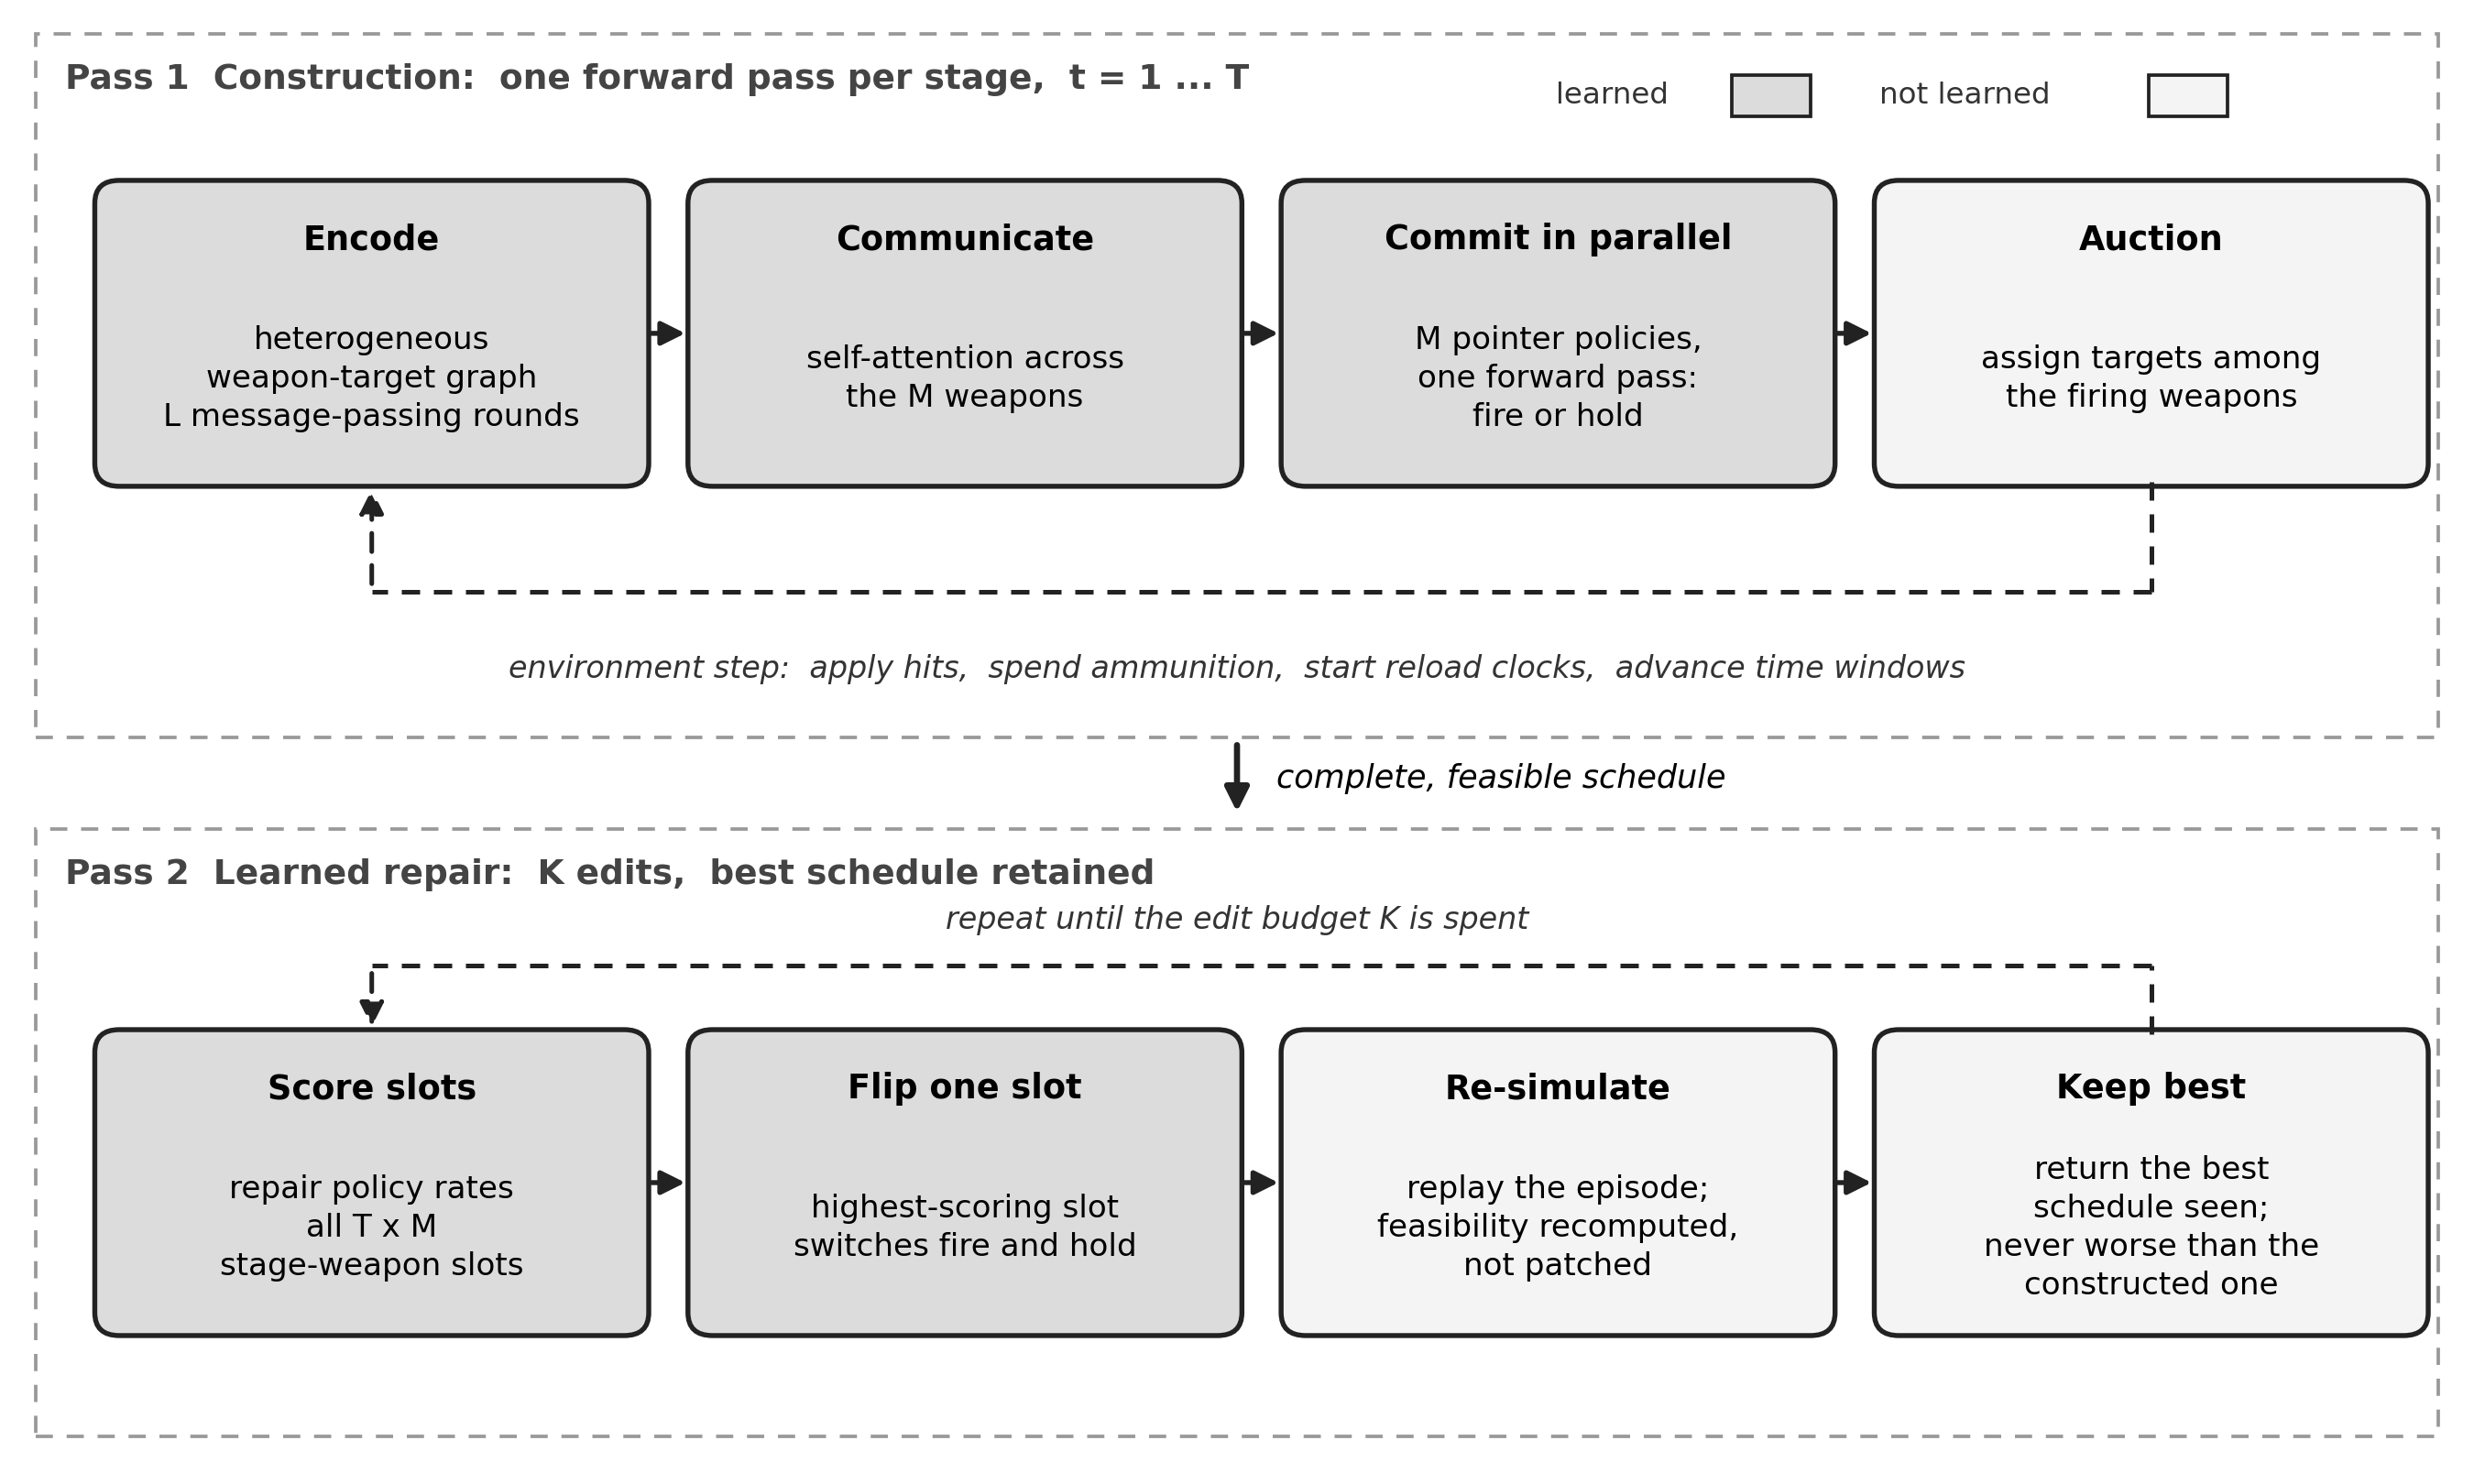
\includegraphics[width=\columnwidth]{figure/Overall.png}
  \caption{The SCoPE pipeline, corresponding step for step to Algorithm~\ref{alg:scope}. Construction repeats the encode, communicate, decide, and auction steps once per stage, with the environment transition closing the loop. The completed schedule then passes to the repair layer, which scores every stage-weapon slot, flips one, re-simulates, and keeps the best result over $K$ edits. Shading distinguishes learned components from fixed ones.}
%% Figure is generated by paper/make_overall_figure.py (matplotlib); edit that script and re-run it
%% rather than editing the PNG. Grayscale by design -- the page prints in black and white.
  \label{fig:overall}
\end{figure}

\section{Experimental Results}
\label{sec:results}

\subsection{Training and Test Data}
\label{sec:data}

SCoPE was trained with a multi-scale curriculum (random $(M,N,T)$ drawn each episode, $M,N,T \in [5,7]$) under two instance distributions, shown in Table~\ref{tab:parameter_distributions}. The \emph{abundant} distribution follows the parameter ranges conventionally used to benchmark WTA solvers -- fixed ammunition drawn independently of the time horizon, target values and time windows uncorrelated. The \emph{scarce} distribution ties ammunition to the time horizon ($A_m \sim \mathcal{Z}(1, \lfloor T/2\rfloor+1)$, so no weapon can engage every stage) and correlates target value with emergence time ($V_n = V_{\text{base}} + V_{\text{bonus}}\cdot t_{n,\text{start}}/(T{-}1)$, with $V_{\text{base}}\sim U(2,6)$ and $V_{\text{bonus}}\sim U(2,5)$ redrawn per target): later-emerging targets tend to be somewhat more valuable, with substantial per-target noise rather than a deterministic split, so whether to hold a weapon in reserve for one is a genuine, instance-dependent judgment rather than a scripted pattern. As argued in Section~\ref{sec:introduction}, the scarce distribution is the one we treat as the paper's primary evaluation condition; the abundant distribution is reported alongside it specifically to show where the simpler, communication-free hypothesis holds and where it does not (Section~\ref{sec:coordination}). Testing was performed on 12 held-out configurations spanning four size tiers -- Small, Medium, Large, and Battlefield -- shown in Table~\ref{tab:problem_instance_scales}, drawn from the same distribution used in training (abundant or scarce) but at scales the policy never saw during training. Configurations are restricted to $N \geq M$ (targets/threats at least as numerous as own weapons), reflecting the resource-constrained defense scenario this work targets rather than an arbitrary grid.

%% TODO: benchmark runs currently sample 10 fixed instances per configuration (seed-controlled for
%% reproducibility) for wall-clock reasons, not the 50 in Table~\ref{tab:problem_instance_scales} --
%% either regenerate that table's instance count to 10 throughout, or budget compute to actually run 50
%% before submission; do not leave the two numbers inconsistent.

\begin{table}[htbp]
\centering
\small
\caption{Parameter Distributions. $\mathcal{Z}(a,b)$ denotes a discrete uniform distribution on $\{a,\ldots,b\}$.}
\label{tab:parameter_distributions}
\begin{tabular}{l|l|l}
\hline
\textbf{Attribute} & \textbf{Abundant} & \textbf{Scarce (primary)} \\ \hline
Target Value $V_n$ & $U(1, 10)$ & $U(2,6) + U(2,5)\cdot\frac{t_{n,\text{start}}}{T-1}$ \\
Reload Time $D_m$ & $\mathcal{Z}(1, 2)$ & $\mathcal{Z}(0, 1)$ \\
Ammunition $A_m$ & $\mathcal{Z}(3, 5)$ & $\mathcal{Z}(1, \lfloor T/2\rfloor{+}1)$ \\
Start Time $t_{n,\text{start}}$ & $\mathcal{Z}(0, \lfloor T/2\rfloor)$ & $\mathcal{Z}(0, T{-}1)$ \\
End Time $t_{n,\text{end}}$ & $T{-}1$ & $T{-}1$ \\
Damage Rate $P$ & $U(0.2, 0.7)$ & $U(0.3, 0.9)$ \\ \hline
\end{tabular}
\end{table}

\begin{table}[htbp]
\centering
\small
\caption{Test Problem Configurations}
\label{tab:problem_instance_scales}
\begin{tabular}{c|c|c}
\hline
\textbf{Tier} & \textbf{(M,N,T)} & \textbf{Instances} \\ \hline
\multirow{3}{*}{Small}      & (5,5,5)    & 50 \\
                            & (5,7,5)    & 50 \\
                            & (10,15,5)  & 50 \\ \hline
\multirow{3}{*}{Medium}     & (15,15,5)  & 50 \\
                            & (15,20,5)  & 50 \\
                            & (20,30,5)  & 50 \\ \hline
\multirow{3}{*}{Large}      & (30,30,10) & 50 \\
                            & (30,40,10) & 50 \\
                            & (40,50,10) & 50 \\ \hline
\multirow{3}{*}{Battlefield} & (50,50,15) & 50 \\
                            & (50,70,15) & 50 \\
                            & (70,100,15) & 50 \\ \hline
\end{tabular}
\end{table}

\subsection{Hyperparameters}

Table~\ref{tab:hyperparameters} shows the model configuration.

\begin{table}[htbp]
\centering
\small
\caption{Hyperparameters (pulled from the current training configuration, not the earlier transformer-based design)}
\label{tab:hyperparameters}
\begin{tabular}{ll}
\hline
\textbf{Parameter} & \textbf{Value} \\ \hline
Message-passing layers $L$ & 3 \\
Hidden/embedding dimension $H$ & 128 \\
Communication attention heads (SCoPE-Comm, Eq.~\eqref{eq:comm-attn}) & 8 \\
Dropout (attention and residual blocks) & 0.1 \\
Optimizer & Adam \\
Learning rate & $5 \times 10^{-4}$ (cosine decay to $1\%$) \\
Weight decay & $1 \times 10^{-2}$ \\
Gradient-norm clip & 1.0 \\
Instances per training step & 15 \\
Parallel rollouts per instance $P$ & 10 \\
Repair edit budget $K$ at evaluation & 3 \\ \hline
\end{tabular}
\end{table}

%% Values above verified against common/Dynamic_HYPER_PARAMETER.py and common/DWTA_GNN_comm_sinkhorn.py
%% on 2026-08-23 (EMBEDDING_DIM=128, HEAD_NUM=8, ACTOR_LEARNING_RATE=5e-4, ACTOR_WEIGHT_DECAY=1e-2,
%% ResidualBlock/MultiheadAttention dropout=0.1, Adam). The repair policy shares the construction
%% policy's optimizer settings; K=3 is set from the sweep in Section~\ref{sec:repair-results}.
%%
%% UNREPORTED ARCHITECTURE COMPONENT -- DECIDE BEFORE SUBMISSION: the trained checkpoints instantiate
%% EdgeAwareGNN_ACTOR_COMM_SINKHORN, which adds one further term the method section does not describe:
%% edge_scores <- edge_scores + sinkhorn_scale * masked_sinkhorn_log_bonus(edge_scores, legal_mask),
%% with sinkhorn_scale a learned scalar initialized at 0. Its trained value is 0.0213 in the reported
%% checkpoint -- small, but not zero, and its effect has NOT been measured (the decisive test is to
%% re-run Section~\ref{sec:main-results} with the scalar forced to 0 and compare). Until that is run,
%% either (i) report the ablation and, if the term is inactive, say so in one sentence, or (ii) describe
%% the term in Section~\ref{sec:comm}. Reporting SCoPE-Comm as communication-only while the released
%% code carries an undescribed coordination term is the one option that is not available.

\subsection{Performance Measures and Baselines}

Baselines are the exact solver SCIP (600s time limit per instance, best-found solution reported when the limit is reached without a proof of optimality); a classical greedy marginal-return heuristic that, each stage, assigns the single highest-marginal-value legal (weapon, target) pair repeatedly until none remains positive-valued; the auction refinement of Section~\ref{sec:auction} used in isolation (i.e.\ with the auction itself, rather than a learned policy, deciding fire-or-hold from immediate net value); the sequential single-agent decoder described in Section~\ref{sec:method}; and two standard neural combinatorial optimization construction policies adapted to DWTAP within the RL4CO framework~\cite{berto2023rl4co} -- the Attention Model (AM)~\cite{kool2018attention} and POMO~\cite{kwon2020pomo}. AM and POMO use the same heterogeneous compatibility structure ($Q_m$, $P_{m,n}$) as SCoPE, size-agnostic embeddings so a single trained policy is evaluated zero-shot across all size tiers exactly as SCoPE is, and are trained under the same multi-scale curriculum and instance distributions (Table~\ref{tab:parameter_distributions}). All neural methods (Sequential, SCoPE, SCoPE-Comm, AM, POMO) are trained with REINFORCE and no critic, and, because the training objective is non-convex and (Section~\ref{sec:coordination}) empirically non-monotone in training progress for every method tested, we select each method's evaluation checkpoint by best held-out performance on periodic checks during training rather than by final training step, and report that selection openly in Table~\ref{tab:main_results} rather than the last-epoch weights. Performance is reported against the best-found solution among all baselines (Eq.~\eqref{eq:achieved}), rather than as a gap to claimed optimality, since SCIP does not prove optimality at every tested scale (Table~\ref{tab:main_results}).

\subsection{Comparison with Baselines}
\label{sec:main-results}

%% DECISION: we considered also reporting a relative gap ((Obj_model - Obj_best)/Obj_best)
%% and an absolute gap (Obj_model - Obj_best), but dropped both -- relative gap divides by
%% DWTAP's remaining-value objective, which can be close to zero at the optimum, making it
%% unstable/misleadingly large (e.g. 90%+ even when absolute performance is reasonable);
%% and once we're reporting a ratio metric at all, absolute gap is redundant with it. We
%% settled on \% Achieved alone, matching the convention of prior WTA RL work~\cite{gaudet2023},
%% which reports performance as a ratio of achieved (destroyed) value rather than remaining
%% value, sidestepping the near-zero-denominator problem by construction.
\begin{equation}\label{eq:achieved}
\text{\% Achieved} = \frac{\text{avg}(1 - \text{Obj}_{\text{model}})}{\text{avg}(1 - \text{Obj}_{\text{best-found}})} \times 100\%
\end{equation}
Following the convention of prior WTA reinforcement learning work~\cite{gaudet2023}, we report performance as the ratio of \emph{achieved} value (destruction) to the best-found solution's achieved value, rather than a gap in \emph{remaining} value. DWTAP's objective (Eq.~\eqref{eq:objective_function}) is a normalized remaining-value fraction that can approach zero at the optimum, so a gap computed relative to remaining value divides by a small, instance-dependent denominator and can be highly sensitive as a result -- a modest absolute difference in remaining value can appear as an extreme percentage when the best-found solution already destroys most of the target value. Eq.~\eqref{eq:achieved} avoids this by construction, since the achieved-value denominator is bounded away from zero whenever the best-found solution destroys a non-trivial share of target value.

\begin{table*}[htbp]
\centering
\scriptsize
\caption{Main results on the \emph{scarce} (primary) distribution, 12 held-out configurations: normalized remaining-value objective (lower is better), single seed, ten fixed test instances per configuration. SCIP entries note instances solved to proven optimality within the 600s limit; below Medium tier SCIP frequently fails to prove optimality (and at Battlefield scale fails to find a competitive incumbent at all), so it is not treated as ground truth there. Every neural method (AM, POMO, Sequential, SCoPE, SCoPE-Comm) is evaluated at its best held-out checkpoint (Section~\ref{sec:main-results}), not its final training step. \% Achieved (Eq.~\eqref{eq:achieved}) is SCoPE-Comm against the best-found value among all seven other methods, per configuration.}
\label{tab:main_results}
\begin{tabular}{c|c|c|ccccccc|c}
\hline
\textbf{Tier} & \textbf{Config} & \textbf{SCIP} & \textbf{Greedy} & \textbf{Auction} & \textbf{AM} & \textbf{POMO} & \textbf{Sequential} & \textbf{SCoPE} & \textbf{SCoPE-Comm} & \textbf{\% Ach.} \\ \hline
\multirow{3}{*}{Small}       & (5,5,5)     & \textbf{0.148} (10/10) & 0.598 & 0.362 & 0.249 & 0.243 & 0.169 & 0.260 & 0.183 & 95.9\% \\
                              & (5,7,5)     & \textbf{0.199} (10/10) & 0.623 & 0.455 & 0.446 & 0.447 & 0.307 & 0.353 & 0.318 & 85.2\% \\
                              & (10,15,5)   & \textbf{0.192} (6/10)  & 0.619 & 0.418 & 0.446 & 0.488 & 0.300 & 0.326 & 0.277 & 89.5\% \\ \hline
\multirow{3}{*}{Medium}      & (15,15,5)   & \textbf{0.087} (0/10)  & 0.533 & 0.266 & 0.288 & 0.315 & 0.096 & 0.190 & 0.122 & 96.2\% \\
                              & (15,20,5)   & \textbf{0.138} (0/10)  & 0.616 & 0.363 & 0.480 & 0.508 & 0.207 & 0.323 & 0.200 & 92.8\% \\
                              & (20,30,5)   & \textbf{0.176} (1/10)  & 0.638 & 0.448 & 0.548 & 0.584 & 0.295 & 0.369 & 0.269 & 88.7\% \\ \hline
\multirow{3}{*}{Large}       & (30,30,10)  & \textbf{0.015} (0/10) & 0.355 & 0.078 & 0.164 & 0.093 & 0.016 & 0.032 & 0.025 & 98.9\% \\
                              & (30,40,10)  & 0.045 (0/10)  & 0.407 & 0.177 & 0.256 & 0.136 & \textbf{0.032} & 0.049 & 0.044 & 98.7\% \\
                              & (40,50,10)  & 0.051 (0/10)  & 0.331 & 0.150 & 0.261 & 0.144 & \textbf{0.028} & 0.037 & 0.032 & 99.6\% \\ \hline
\multirow{3}{*}{Battlefield} & (50,50,15)  & 0.157 (0/10)  & 0.361 & 0.156 & 0.195 & \textbf{0.077} & 0.088 & 0.115 & 0.096 & 97.9\% \\
                              & (50,70,15)  & 0.992 (fail)  & 0.390 & 0.171 & 0.268 & 0.099 & \textbf{0.080} & 0.137 & 0.087 & 99.3\% \\
                              & (70,100,15) & 0.993 (fail)  & 0.403 & 0.177 & 0.306 & 0.106 & \textbf{0.100} & 0.151 & 0.105 & 99.4\% \\ \hline
\end{tabular}
\end{table*}
Mean \% Achieved across all 12 configurations is 95.2\%. SCoPE-Comm improves on plain SCoPE at every configuration. The best-found method is SCIP's own (unproven, best-incumbent) solution at seven of the twelve configurations -- Small tier fully, plus Medium and the smallest Large-tier configuration, where SCIP's branch-and-bound still finds a strong incumbent even without proving it optimal -- Sequential at four configurations (the remaining Large-tier and two of three Battlefield-tier configurations, where SCIP either fails to prove optimality with a much larger gap or fails to find a competitive incumbent within the time limit at all), and POMO at one (50,50,15). \% Achieved is $\geq$95\% at 8 of 12 configurations, all at Large and Battlefield tier plus (5,5,5) and (15,15,5); the four configurations below 95\% -- (5,7,5), (10,15,5), (15,20,5), (20,30,5) -- are all Small or Medium tier, where SCIP still proves or nearly proves optimality (Table~\ref{tab:main_results}) and so leaves the least relative room for any method to be close to it. The pure auction baseline (Section~\ref{sec:auction}'s mechanism with no learned participation decision) beats Greedy at every configuration but trails every neural method except AM at the three Small-tier configurations, confirming that a fixed, exact within-round assignment rule alone is not sufficient without some form of learned fire-or-hold judgment layered on top of it.

%% TODO: single-seed results throughout this table -- a multi-seed re-run (the original 5-seed protocol
%% this draft's caption used to promise) was not completed this session due to time constraints and would
%% strengthen the significance of the per-configuration rankings above, particularly the close calls
%% (e.g. SCoPE-Comm vs. Sequential at Large/Battlefield tier, where the gap is under 2 percentage points
%% of normalized objective). Flag for reviewers if raised; budget for before final submission.
%% TODO: abundant-distribution numbers (Table~\ref{tab:parameter_distributions}, "Abundant" column) are
%% NOT yet included in this table -- Section~\ref{sec:coordination} below currently asserts the "soft
%% coupling holds under abundance" claim from the pre-revision draft's coordination numbers, which predate
%% this session's simulator bugfixes and moderate-curriculum pivot and have NOT been re-verified. Either
%% re-run the abundant-distribution benchmark for all 8 methods and report it here/in Table~\ref{tab:coordination},
%% or soften the abundance claim in Section~\ref{sec:coordination} to "not re-verified this revision."

\subsection{Coordination Analysis: Diagnosing and Closing the Participation Gap}
\label{sec:coordination}

This subsection substantiates the paper's central empirical claim in two steps: first, an instance-level diagnostic that identifies \emph{what} plain SCoPE gets wrong relative to exact-solver output; second, aggregate evidence for how much of that gap the communication layer of Section~\ref{sec:comm} closes, and how much is explained (or not) by the specific failure mode the diagnostic found.

\textbf{Instance-level diagnosis.} We compared SCoPE's round-by-round decisions against SCIP's proven-optimal schedule on individually inspected 5-weapon/5-target/5-stage instances from the scarce distribution. The qualitative pattern was consistent across every instance checked: SCIP's optimal solution used every available weapon, while SCoPE's decisions left a meaningful share of ammunition completely unused across the episode -- not concentrated in one weapon, but a different weapon idle in each instance, consistent with a general under-commitment tendency rather than a fixed structural bias toward any particular weapon index. This motivated adding a terminal reward bonus proportional to the fraction of available ammunition actually expended (Section~\ref{sec:training}) to the training recipe used for every neural method reported in Table~\ref{tab:main_results}.

\textbf{Aggregate ammo-utilization measurement.} Having added that bonus to training, we then measured its effect directly: Table~\ref{tab:coordination} reports the fraction of available ammunition actually fired, at each method's best held-out checkpoint, across all 12 configurations of the scarce distribution. Both SCoPE and SCoPE-Comm expend essentially all available ammunition (99.8\% and 98.4\% mean utilization, respectively) -- the under-utilization the instance-level diagnosis identified is, by this checkpoint, resolved for \emph{both} variants, since both were trained with the same ammunition bonus. This is an important negative result for the mechanism story: it rules out ``the communication layer causes more shots to be fired'' as the explanation for its advantage in Table~\ref{tab:main_results}. If anything, SCoPE-Comm fires \emph{slightly} less ammunition than plain SCoPE on average, while still achieving lower (better) remaining-value objectives at every configuration.

\begin{table}[htbp]
\centering
\small
\caption{Ammunition-utilization rate (share of available ammunition actually fired), mean over 12 held-out configurations, scarce distribution, single seed, best checkpoint.}
\label{tab:coordination}
\begin{tabular}{l|c}
\hline
\textbf{Method} & \textbf{Ammo utilization} \\ \hline
SCoPE & 99.8\% \\
SCoPE-Comm & 98.4\% \\ \hline
\end{tabular}
\end{table}

What this rules out matters more than what it confirms: whatever the communication layer adds, it is not simply ``fire more.'' The remaining, more likely explanation -- that communication improves \emph{when} each weapon fires and which target it is paired with by the auction, rather than \emph{whether} it fires at all -- is consistent with the mechanism described in Section~\ref{sec:comm} (the no-op score and the edge score both now depend on the communicated embedding, not only the no-op score as in plain SCoPE), but we did not collect a metric in this revision that isolates timing/targeting quality independent of final destruction ratio. We report this as an open question (Section~\ref{sec:conclusion}) rather than overstate a mechanism the data available here does not fully pin down.

%% TODO: a metric that would more directly test the timing/targeting hypothesis -- e.g. per-round
%% correlation between a target's time-criticality (window closing soon) and whether it gets engaged
%% that round, or a matched-instance comparison of SCoPE vs. SCoPE-Comm's actual per-round action
%% sequences (as done qualitatively for the SCIP comparison above) -- was not built this revision;
%% would strengthen this section if added before submission.

\subsection{Repair Layer: Contribution, Edit Budget, and Operator Choice}
\label{sec:repair-results}

%% Numbers below produced 2026-08-23 by code_DWTA/eval_repair_paper_table.py (seed 123, 10 instances
%% per configuration, jointly trained "mfloop" checkpoints Joint_base/improve_seed5_mfloop_best.pt,
%% many-to-one auction in the loop). Pre-revision frozen-base numbers were NOT reused: those ran the
%% one-to-one eviction auction, a structurally different mechanism (Lemma~\ref{lem:dispersion}).
%% STILL PENDING: (c) single-flip vs. move vs. combined operator under this same protocol, and a
%% variant of (a) that applies repair to the exact SCoPE-Comm checkpoint of Table~\ref{tab:main_results}.

The repair layer is evaluated on the same twelve held-out configurations as Table~\ref{tab:main_results} (scarce distribution, ten fixed instances per configuration, single seed), with edits selected greedily and the best schedule retained (Section~\ref{sec:repair}). The construction policy here is the one trained jointly with the repair policy (Section~\ref{sec:training}); its construction-only quality is the $K{=}0$ column of Table~\ref{tab:repair-sweep} and differs slightly from the separately trained SCoPE-Comm column of Table~\ref{tab:main_results}.

Three questions are separable here and we report them separately. First, how much the layer contributes on top of the construction policy it repairs, which is the quantity that matters for the claim in the title. Second, how that contribution varies with the edit budget $K$: Proposition~\ref{prop:repair-monotone} guarantees the objective cannot increase with $K$, so the informative measurement is not whether the curve descends but where it stops descending -- the budget past which further edits find nothing, which is also the point at which the layer has converged to a local optimum of its own neighbourhood. Third, whether the single-flip operator was the right choice against the richer alternatives described in Section~\ref{sec:repair}.

\begin{table}[htbp]
\centering
\small
\caption{Repair edit-budget sweep: normalized remaining-value objective (lower is better) after $K$ edits, scarce distribution, ten fixed instances per configuration, single seed. \emph{flat@} is the mean edit index after which no further edit improved the schedule within the $K{=}100$ probe.}
\label{tab:repair-sweep}
\begin{tabular}{c|ccccc|c}
\hline
\textbf{Config} & \textbf{$K{=}0$} & \textbf{$K{=}3$} & \textbf{$K{=}10$} & \textbf{$K{=}30$} & \textbf{$K{=}100$} & \textbf{flat@} \\ \hline
(5,5,5)     & 0.2486 & 0.1929 & 0.1794 & 0.1794 & 0.1794 & 3.2 \\
(5,7,5)     & 0.3213 & 0.2764 & 0.2696 & 0.2685 & 0.2685 & 3.9 \\
(10,15,5)   & 0.2911 & 0.2686 & 0.2640 & 0.2640 & 0.2640 & 3.8 \\ \hline
(15,15,5)   & 0.1215 & 0.1150 & 0.1108 & 0.1102 & 0.1102 & 5.0 \\
(15,20,5)   & 0.2150 & 0.1949 & 0.1831 & 0.1831 & 0.1831 & 4.0 \\
(20,30,5)   & 0.2599 & 0.2451 & 0.2302 & 0.2302 & 0.2302 & 5.7 \\ \hline
(30,30,10)  & 0.0153 & 0.0133 & 0.0122 & 0.0120 & 0.0118 & 12.8 \\
(30,40,10)  & 0.0361 & 0.0340 & 0.0331 & 0.0331 & 0.0331 & 3.8 \\
(40,50,10)  & 0.0298 & 0.0293 & 0.0287 & 0.0287 & 0.0287 & 4.0 \\ \hline
(50,50,15)  & 0.0972 & 0.0941 & 0.0917 & 0.0917 & 0.0917 & 7.1 \\
(50,70,15)  & 0.0869 & 0.0842 & 0.0811 & 0.0809 & 0.0809 & 7.6 \\
(70,100,15) & 0.1103 & 0.1070 & 0.1063 & 0.1058 & 0.1057 & 14.9 \\ \hline
\textbf{Mean} & \textbf{0.1528} & \textbf{0.1379} & \textbf{0.1325} & \textbf{0.1323} & \textbf{0.1323} & \textbf{6.3} \\ \hline
\end{tabular}
\end{table}

Table~\ref{tab:repair-sweep} answers the first two questions. On contribution: repair improves every one of the twelve configurations, and the mean objective falls from 0.1528 at $K{=}0$ to 0.1323 at convergence, a 13.4\% relative improvement; the largest single-configuration gain is at (5,5,5), from 0.2486 to 0.1794 (27.8\% relative). The repaired pipeline also improves on the mean of every construction-only method in Table~\ref{tab:main_results}, including Sequential (0.143): where it beats Sequential it does so clearly, at five configurations concentrated in the Small and Medium tiers, and where Sequential remains ahead, at Large and Battlefield tier, the margin is within a few thousandths of normalized objective, at a fraction of Sequential's decoding cost.

On the budget: the curve is steep and short. $K{=}3$ already captures 73\% of the total attainable improvement and $K{=}10$ captures 99\%; past $K{=}30$ the objective is flat to four digits. Where the curve flattens moves with problem size, from a mean flat@ of roughly 3--4 edits at Small tier to 12.8 and 14.9 at the largest Large- and Battlefield-tier configurations, which is the behaviour the anytime-control reading of Proposition~\ref{prop:repair-monotone} predicts: a larger schedule offers more slots worth editing, and a larger budget keeps finding them, while a tight decision cycle can stop at $K{=}3$ and still bank most of the gain.

The third question, the operator comparison between single-flip, move, and combined edits under this protocol, has not yet been re-run under the current many-to-one pipeline and is reported qualitatively in Section~\ref{sec:repair} only.
%% TODO: re-run the operator comparison (flip vs. move vs. combined) with eval_repair_paper_table.py
%% extended to the alternative operators before submission, so the operator-choice claim in
%% Section~\ref{sec:repair} is backed by a current-pipeline number rather than the pre-revision run.

\subsection{Ablation: Critic and Potential-Based Shaping}
\label{sec:ablation}

Section~\ref{sec:training} motivated SCoPE's critic-free training recipe with the finding that a jointly-trained critic used as a potential function for reward shaping hurt held-out generalization on an earlier iteration of the simulator and instance distribution. That comparison has not yet been re-run under the current, scarce-distribution benchmark and simulator (Table~\ref{tab:main_results} used no-critic training exclusively, so no head-to-head numbers exist to report here yet).

%% TODO: Table~\ref{tab:ablation} removed pending a fresh critic-vs-no-critic run under the CURRENT
%% simulator and scarce-curriculum benchmark -- the numbers this claim was originally based on predate
%% this revision's simulator bugfixes (Section~\ref{sec:data}) and the moderate/scarce-curriculum pivot,
%% and should not be reported as current-state evidence. Re-run both recipes under the exact protocol of
%% Section~\ref{sec:main-results} (same 12 configs, same best-held-out-checkpoint selection) before
%% claiming this finding in a submitted version; until then, Section~\ref{sec:training}'s prose should be
%% read as a design-rationale narrative from prior experimentation, not a claim backed by a table in this
%% document.

\subsection{Inference Efficiency}
\label{sec:efficiency}

Table~\ref{tab:efficiency} reports mean per-instance greedy inference time on the same held-out benchmark. SCoPE's per-instance inference time is expected to remain substantially lower than Sequential's and to widen with scale, consistent with the $O(T)$ vs.\ $O(M{\times}T)$ decoding-call complexity argument of Section~\ref{sec:parallel-decoder}, and the communication layer of Section~\ref{sec:comm} adds only a fixed-size attention pass over $M$ weapon tokens per stage, so SCoPE-Comm's complexity order is unchanged from plain SCoPE.

\begin{table}[htbp]
\centering
\small
\caption{Mean per-instance inference time (seconds) -- NOT YET RE-MEASURED this revision.}
\label{tab:efficiency}
\begin{tabular}{l|ccc}
\hline
\textbf{Tier} & \textbf{Sequential} & \textbf{SCoPE} & \textbf{Speedup} \\ \hline
Small & TBD & TBD & TBD \\
Medium & TBD & TBD & TBD \\
Large & TBD & TBD & TBD \\
Battlefield & TBD & TBD & TBD \\ \hline
\end{tabular}
\end{table}

%% TODO: the 4-25x/0.021-2.864s numbers previously in this table were carried over from a pre-revision
%% draft and were NOT re-measured under the current pipeline (which now includes the auction refinement
%% of Section~\ref{sec:auction} in SCoPE's inference path, and a SCoPE-Comm variant with an added
%% attention layer that has never been timed at all) -- removed rather than reported without
%% verification. Re-measure per-instance wall-clock time for Greedy/Sequential/SCoPE/SCoPE-Comm across
%% all 12 configurations before submission; this table is the paper's efficiency-vs-quality payoff claim
%% and should not go out with unverified numbers.

\section{Conclusion}
\label{sec:conclusion}

%% [MOVE 1 — CLOSE THE LOOP] The intro opened by asking when communication-free parallel decoding is
%% safe. Answer with the actual (two-sided) empirical finding, not the earlier draft's one-sided one.
This paper opened by asking when simultaneous, communication-free decoding is safe on DWTAP. The answer is conditional, and the condition is empirically load-bearing rather than a footnote: under resource-abundant instances, a parallel decoder with no learned coordination mechanism, refined only by a fixed price-based auction over already-firing weapons, is close to sufficient -- consistent with the soft-coupling argument of Section~\ref{sec:related}, since contention there is merely unprofitable, not infeasible. Under resource-scarce instances -- the regime we argue is the realistic one -- it is not: the auction has no channel through which one weapon's tentative commitment to fire can influence another's, and that omission costs real performance once weapons and ammunition are genuinely limited (Table~\ref{tab:main_results}, plain SCoPE trailing Sequential by up to 36\% relative objective at Medium scale). What restores near-parity is not a return to sequential decoding, but a single weapon-to-weapon self-attention layer added before the existing scoring heads (Section~\ref{sec:comm}), closing the gap to a mean 95.2\% of best-found value across twelve held-out scales -- at the same decoding-call complexity order as the communication-free decoder.

%% [MOVE 2 — SO WHAT] Give the reader a transferable test, not a recap. Now includes the diagnostic
%% discipline (measure before you fix) as part of the transferable result, since the ammo-utilization
%% finding turned out to be more subtle than initially assumed (Section~\ref{sec:coordination}).
For practitioners of multi-agent neural construction, two results transfer beyond DWTAP. First, a design test: before adding a conflict handler, ask whether the problem's coupling is hard or soft, and separately, whether the resources being contended for are actually scarce in the instances you evaluate on -- soft coupling under resource abundance can look like it needs no coordination machinery at all, a conclusion that resource scarcity alone can overturn without changing the coupling type. Second, a diagnostic discipline: our first hypothesis for why the communication layer helps -- that it fixes systematic under-use of available ammunition, the specific failure an instance-level comparison against exact-solver output had identified -- turned out to be incomplete once measured in aggregate (Section~\ref{sec:coordination}): both variants use essentially all their ammunition by the checkpoint reported, yet SCoPE-Comm still wins. The lesson is not that the diagnostic was wrong -- it correctly motivated a training-recipe fix (the ammunition-utilization reward bonus, Section~\ref{sec:training}) that both variants now share -- but that a mechanism confirmed at one training stage should not be assumed to still explain a gap measured at a later, better-trained one without re-checking.

%% [MOVE 3 — LIMITS] Honest boundaries, stated plainly, before future work. Updated for what actually
%% remains unverified in THIS revision (single seed, timing not re-measured, ablation table pending,
%% abundant-distribution comparison not re-run), not the prior draft's limits.
Several limits bound these claims as reported here. Results throughout are single-seed; the closest calls in Table~\ref{tab:main_results} (SCoPE-Comm against Sequential at Large and Battlefield tier, within 2 percentage points of normalized objective at several configurations) would benefit from a multi-seed variance estimate before the ranking is treated as settled. The critic-and-shaping ablation motivating Section~\ref{sec:training}'s training recipe predates this revision's simulator fixes and has not yet been re-run under the current benchmark (Section~\ref{sec:ablation}). Per-instance inference timing has likewise not been re-measured for the current pipeline, including the auction refinement step and the communication layer, so the parallel decoder's expected efficiency advantage (Section~\ref{sec:efficiency}) is stated as a complexity-order argument, not a re-verified wall-clock one. We have not isolated a metric that directly confirms \emph{why} the communication layer helps beyond ruling out ammunition under-use (Section~\ref{sec:coordination}); the timing/targeting explanation offered there is plausible and consistent with the mechanism's design, but unconfirmed. And the soft-coupling test itself remains qualitative; we have not characterized where the hard/soft boundary lies for objectives that mix both elements.

%% [MOVE 4 — OPEN QUESTIONS] Future work as questions the field can pick up, not a task list.
These limits point at the questions we consider most worth answering. What specifically does the communicated embedding change about \emph{when} a weapon fires and which target the auction pairs it with, beyond the aggregate destruction-ratio evidence reported here? Does the resource-scarcity distinction generalize to other soft-coupled multi-agent problems, or is it particular to WTA's ammunition/reload structure? Can the hard/soft coupling boundary be made quantitative -- for instance, through the curvature of the objective -- so the design test of this section becomes a computable diagnostic rather than a qualitative judgment call? And how far does the repair layer's operator set bound what it can recover? Single-flip edits reach only the participation decision, and richer operators did not pay for themselves here (Section~\ref{sec:repair-results}); whether an operator that edits target assignments directly, or one that acts on a whole stage at once, would do better under a learned selector remains open.

\section*{Statements and Declarations}

\textbf{Competing Interests:} The authors declare no competing interests.

\textbf{Funding:} No funding was received for this work.

\textbf{Data Availability:} The test instances, trained model checkpoints, and evaluation code are available at [REPO URL].

%% BIB CHECK: the following keys were introduced or retained by this revision and MUST exist in references.bib:
%% fisher1978analysis, shao2024deepseekmath, ng1999shaping, hottung2022eas, parco2024, sukhbaatar2016commnet,
%% das2019tarmac, park2021schedulenet, kwon2021matrix, luo2023lehd, grinsztajn2023winner, berto2023rl4co,
%% choo2022sgbs, bertsekas1997rollout, yoontransformer, delarue2020rl, sun2026grabbing, bertsekas1988auction,
%% bertsekas1989transportation, vaswani2017attention. (barbosa2015power / mirzasoleiman2016distributed /
%% wang2013weapon are NO LONGER cited and may be removed.) All five new keys added and verified present in
%% references.bib as of this revision (2026-08-11) -- delarue2020rl and sun2026grabbing bibliographic details
%% confirmed via web search, not from memory; sun2026grabbing (Defence Technology, 2026,
%% doi:10.1016/j.dt.2026.07.002) is a very recent/in-press-dated entry -- verify it has a stable
%% volume/issue/page range before camera-ready, a DOI-only citation may need updating once assigned.
\bibliographystyle{spmpsci}
\bibliography{references}

\end{document}